\documentclass[cs4size,a4paper,10pt]{ctexart}   

\linespread{1.5}
\usepackage{geometry}%用于设置上下左右页边距
	\geometry{left=2.5cm,right=2.5cm,top=3.2cm,bottom=2.7cm}
\usepackage{xeCJK,amsmath,paralist,enumerate,booktabs,multirow,graphicx,subfig,setspace,listings,lastpage,hyperref}
\usepackage{amsthm, amssymb, bm, color, framed, graphicx, hyperref, mathrsfs}
\usepackage{mathrsfs}  
	\setlength{\parindent}{2em}
	\lstset{language=Matlab}%
\usepackage{fancyhdr}
\usepackage{graphicx}
\usepackage{listings}
\usepackage{xcolor}
\usepackage{float}
\usepackage{paralist}
\usepackage{setspace}
\usepackage{titlesec}
\usepackage{enumitem}
\usepackage{hyperref}



\hypersetup{
	colorlinks=true,
	linkcolor=black
}

\setenumerate{partopsep=0pt,topsep=0pt}
\setitemize{itemsep=0pt,partopsep=0pt,topsep=0pt}

\titlespacing*{\section}{0pt}{3pt}{3pt}
\titlespacing*{\subsection}{0pt}{2pt}{2pt}
\titlespacing*{\subsubsection}{0pt}{1pt}{1pt}
\titlespacing*{\paragraph}{0pt}{0pt}{0pt}

\ctexset{secnumdepth=4,tocdepth=4}
\setlength{\parindent}{0pt}
\setstretch{1.2}


\setCJKmainfont[BoldFont={FZHei-B01},ItalicFont={FZKai-Z03}]{FZShuSong-Z01} 
\setCJKsansfont[BoldFont={FZHei-B01}]{FZKai-Z03} 
\setCJKmonofont[BoldFont={FZHei-B01}]{FZFangSong-Z02}
\setCJKfamilyfont{zhsong}{FZShuSong-Z01} 
\setCJKfamilyfont{zhhei}{FZHei-B01} 
\setCJKfamilyfont{zhkai}[BoldFont={FZHei-B01}]{FZKai-Z03} 
\setCJKfamilyfont{zhfs}[BoldFont={FZHei-B01}]{FZFangSong-Z02} 
\renewcommand*{\songti}{\CJKfamily{zhsong}} 
\renewcommand*{\heiti}{\CJKfamily{zhhei}} 
\renewcommand*{\kaishu}{\CJKfamily{zhkai}} 
\renewcommand*{\fangsong}{\CJKfamily{zhfs}}


\definecolor{mKeyword}{RGB}{0,0,255}          % bule
\definecolor{mString}{RGB}{160,32,240}        % purple
\definecolor{mComment}{RGB}{34,139,34}        % green
\definecolor{mNumber}{RGB}{128,128,128} 

\lstdefinestyle {njulisting} {
	basewidth = 0.5 em,
	lineskip = 3 pt,
	basicstyle = \small\ttfamily,
	% keywordstyle = \bfseries,
	commentstyle = \itshape\color{gray}, 
	basicstyle=\small\ttfamily,
	keywordstyle={\color{mKeyword}},     % sets color for keywords
	stringstyle={\color{mString}},       % sets color for strings
	commentstyle={\color{mComment}},     % sets color for comments
	numberstyle=\tiny\color{mNumber},
	numbers = left,
	captionpos = t,
	breaklines = true,
	xleftmargin = 2 em,
	xrightmargin = 2 em,
	frame=tlrb,
	tabsize=4
}

\lstset{
style = njulisting, % 调用上述样式 
flexiblecolumns % 允许调整字符宽度
}


%================= 基本格式预置 ===========================
\usepackage{fancyhdr}
\pagestyle{fancy}
\lhead{\textsc{Operating System}}
\rhead{第一章\ 计算机操作系统概述}
\cfoot{\thepage}
\renewcommand{\headrulewidth}{0.4pt}
\renewcommand{\theenumi}{(\arabic{enumi})}
\CTEXsetup[format={\bfseries\zihao{-3}}]{section}
\CTEXsetup[format={\bfseries\zihao{4}}]{subsection}
\CTEXsetup[format={\bfseries\zihao{-4}}]{subsubsection}


\renewcommand{\contentsname}{目录}  
\begin{document}

	\begin{center}
		{\huge\textbf{第一章\ 计算机操作系统概述}}
	\end{center}
	%---------目录---------% 
	\pagenumbering{Roman}
	\tableofcontents
	\clearpage

 	%---------正文---------% 
	\pagenumbering{arabic}
	\setcounter{page}{1}
	\setlength{\parskip}{0.65em}
	

	\section{计算机系统}
	\subsection{计算机系统概述}
	\subsubsection{电子数字计算机}
	\begin{itemize}
		\item 电子数字计算机,是一种能够自行按照已设定的程序进行数据处理的电子设备
		\item 电子数字计算机,是软件与硬件相结合、面向系统、侧重应用的自动化求解工具
	\end{itemize}


	\subsubsection{计算机技术的发展}
	计算机的诞生与发展经历了以下几个阶段
	\begin{itemize}
		\item 1945$-$:电子真空管、机器语言,应用于科学计算
		\item 1956$-$:晶体管、批处理控制、Fortran/COBOL,扩展到数据处理领域
		\item 1959$-$:集成电路、多道程序、操作系统/数据库/高级语言,应用领域继续扩展
		\item 1976$-$:大规模/超大规模集成电路,向快速化/小型化/系统化/网络化/智能化等方面发展
		\item 1980$-$:微机出现,廉价化促使应用领域快速膨胀
		\item 1990$-$:图形化人机交互技术,友善化推动了应用人群的快速扩展
		\item 2003$-$:移动计算的出现,计算无处不在
	\end{itemize}

	
	\subsubsection{计算机系统的组成}
	现代计算机系统包括硬件子系统和软件子系统
	\begin{itemize}
		\item 硬件:借助电、磁、光、机械等原理构成的各种物理部件的有机组合,是系统工作的实体
			\begin{itemize}
			\item 包括 CPU,主存储器,I/O 控制系统,外围设备
			\end{itemize}
		\item 软件:各种程序和文件,用于指挥计算机系统按指定的要求进行协同工作
			\begin{itemize}
				\item 包括系统软件、支撑软件和应用软件
				\item 其中最关键的系统软件是操作系统与语言处理程序
			\end{itemize}
	\end{itemize}
	
	

	\subsubsection{计算机系统的用户视图}
	\begin{figure}[ht]
		\centering
		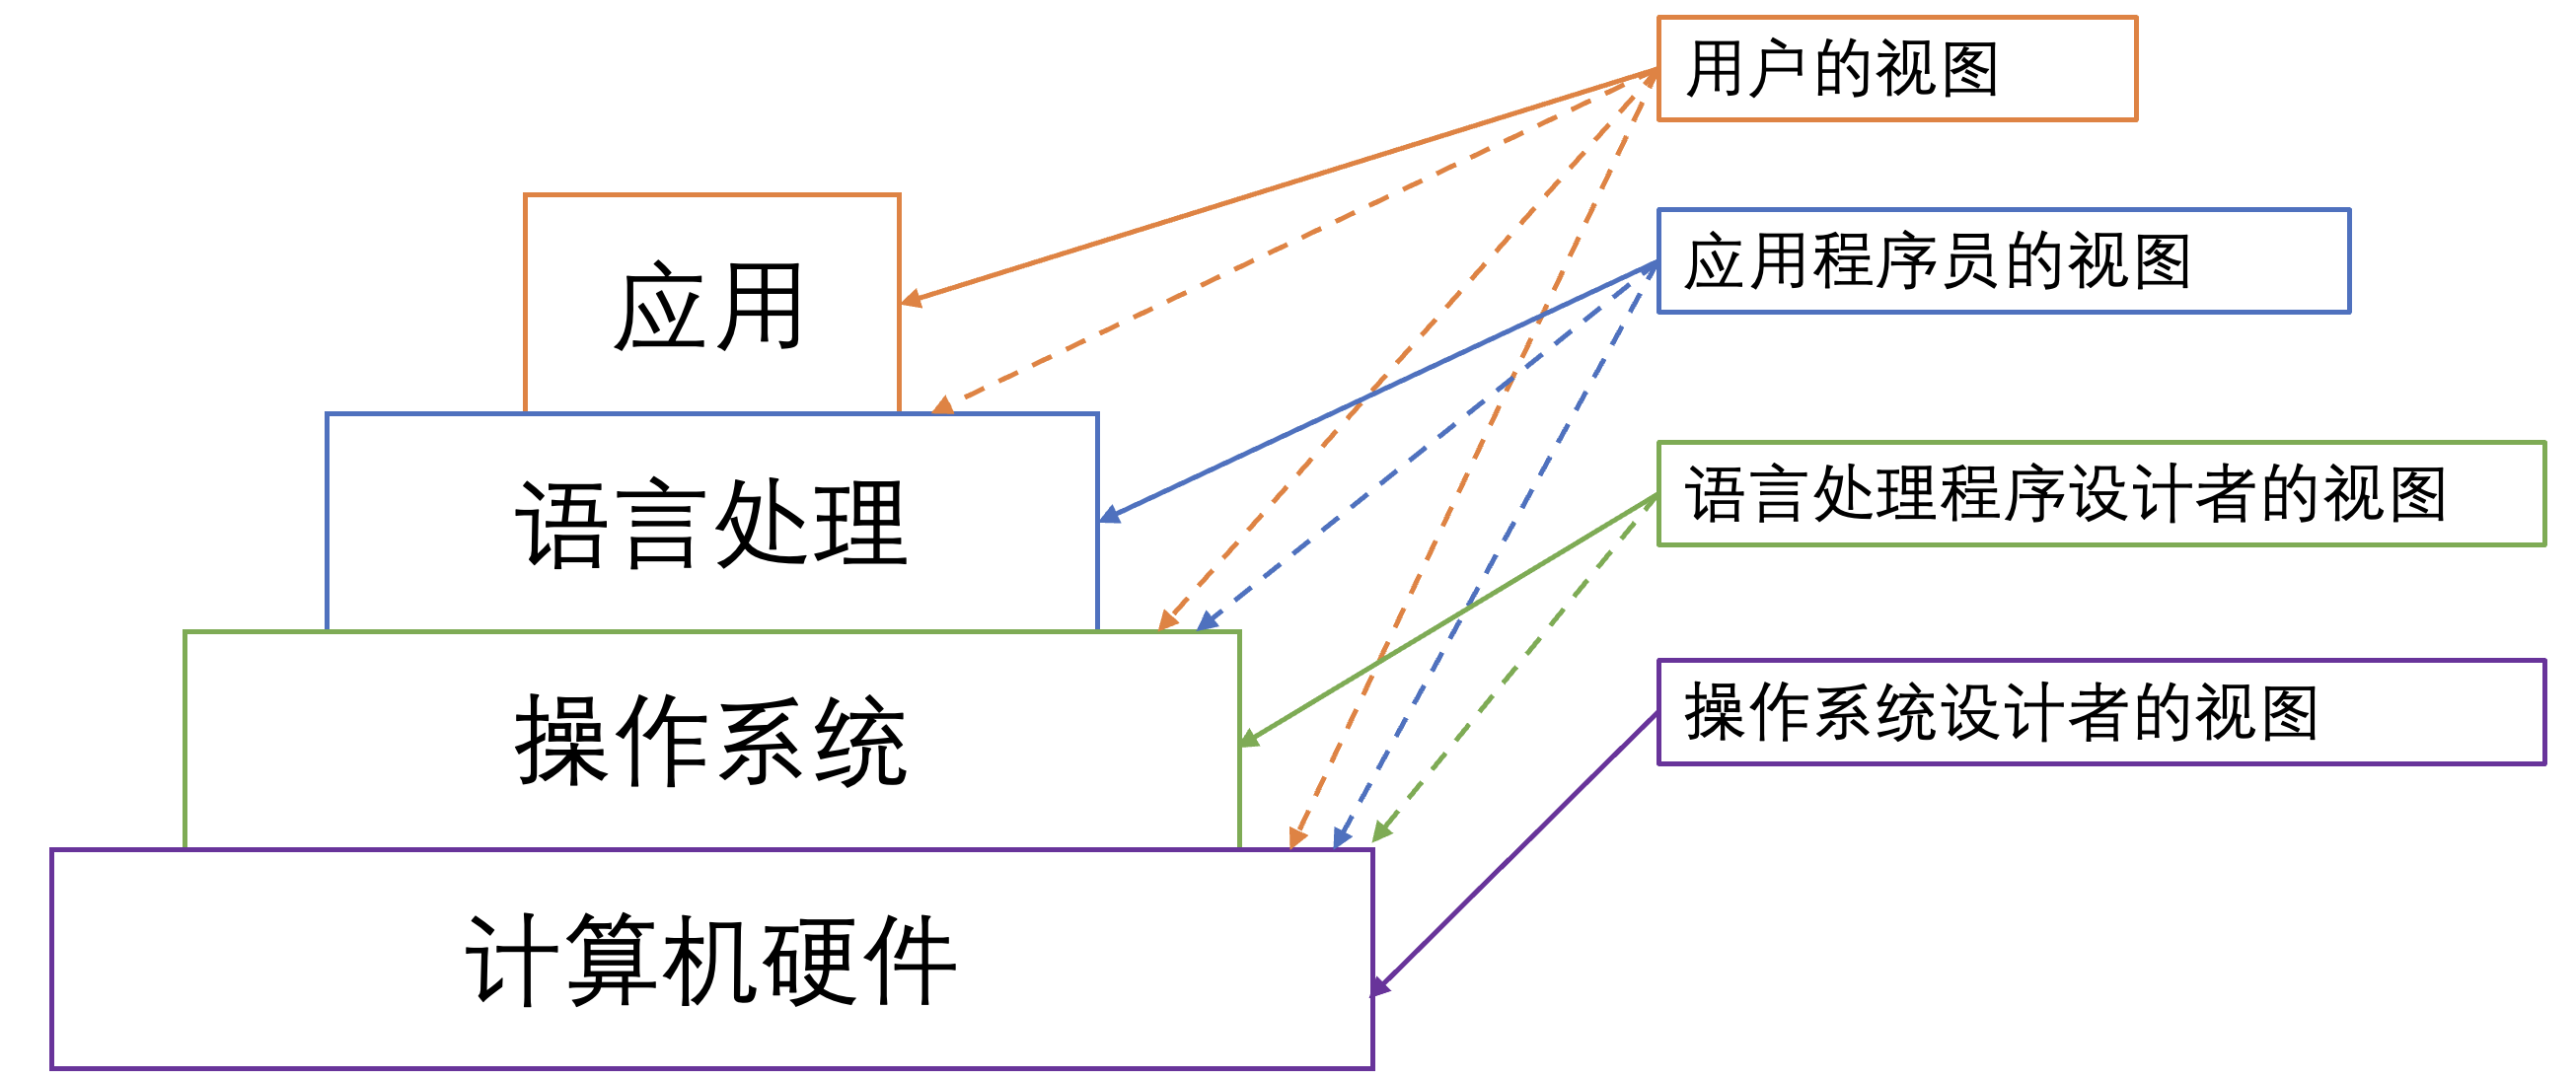
\includegraphics[width=0.6\textwidth]{img/1.1.1.4}
	\end{figure}


	\subsection{计算机硬件系统}
	\subsubsection{计算机硬件系统的组成}
	计算机硬件系统包括中央处理器、主存储器和外围设备等组件,他们通过系统总线连接
	\begin{itemize}
		\item 中央处理器包括运算单元和控制单元
		\begin{itemize}
			\item 运算单元用于执行具体的机器指令的运算
			\item 控制单元用于解译机器指令
		\end{itemize}
		\item 主存储器用于存储正在执行的程序和数据
		\item 外围设备包括输入设备、输出设备、存储设备和网络通信设备
	\end{itemize}

	
	\subsubsection{冯·诺依曼模型}
	当今绝大部分计算机都是基于冯·诺依曼等人在 1946 年提出的存储程序计算机模型,该体系结构的特点为:
	\begin{enumerate}[label=\arabic*.]
		\item 以运算单元为中心,控制流由指令流产生
		\item 采用存储程序原理,面向主存组织数据流
		\item 主存是按地址访问、线性编址的空间
		\item 指令由操作码和地址码组成
		\item 数据以二进制编码
	\end{enumerate}
	\begin{figure}[H]
		\centering
		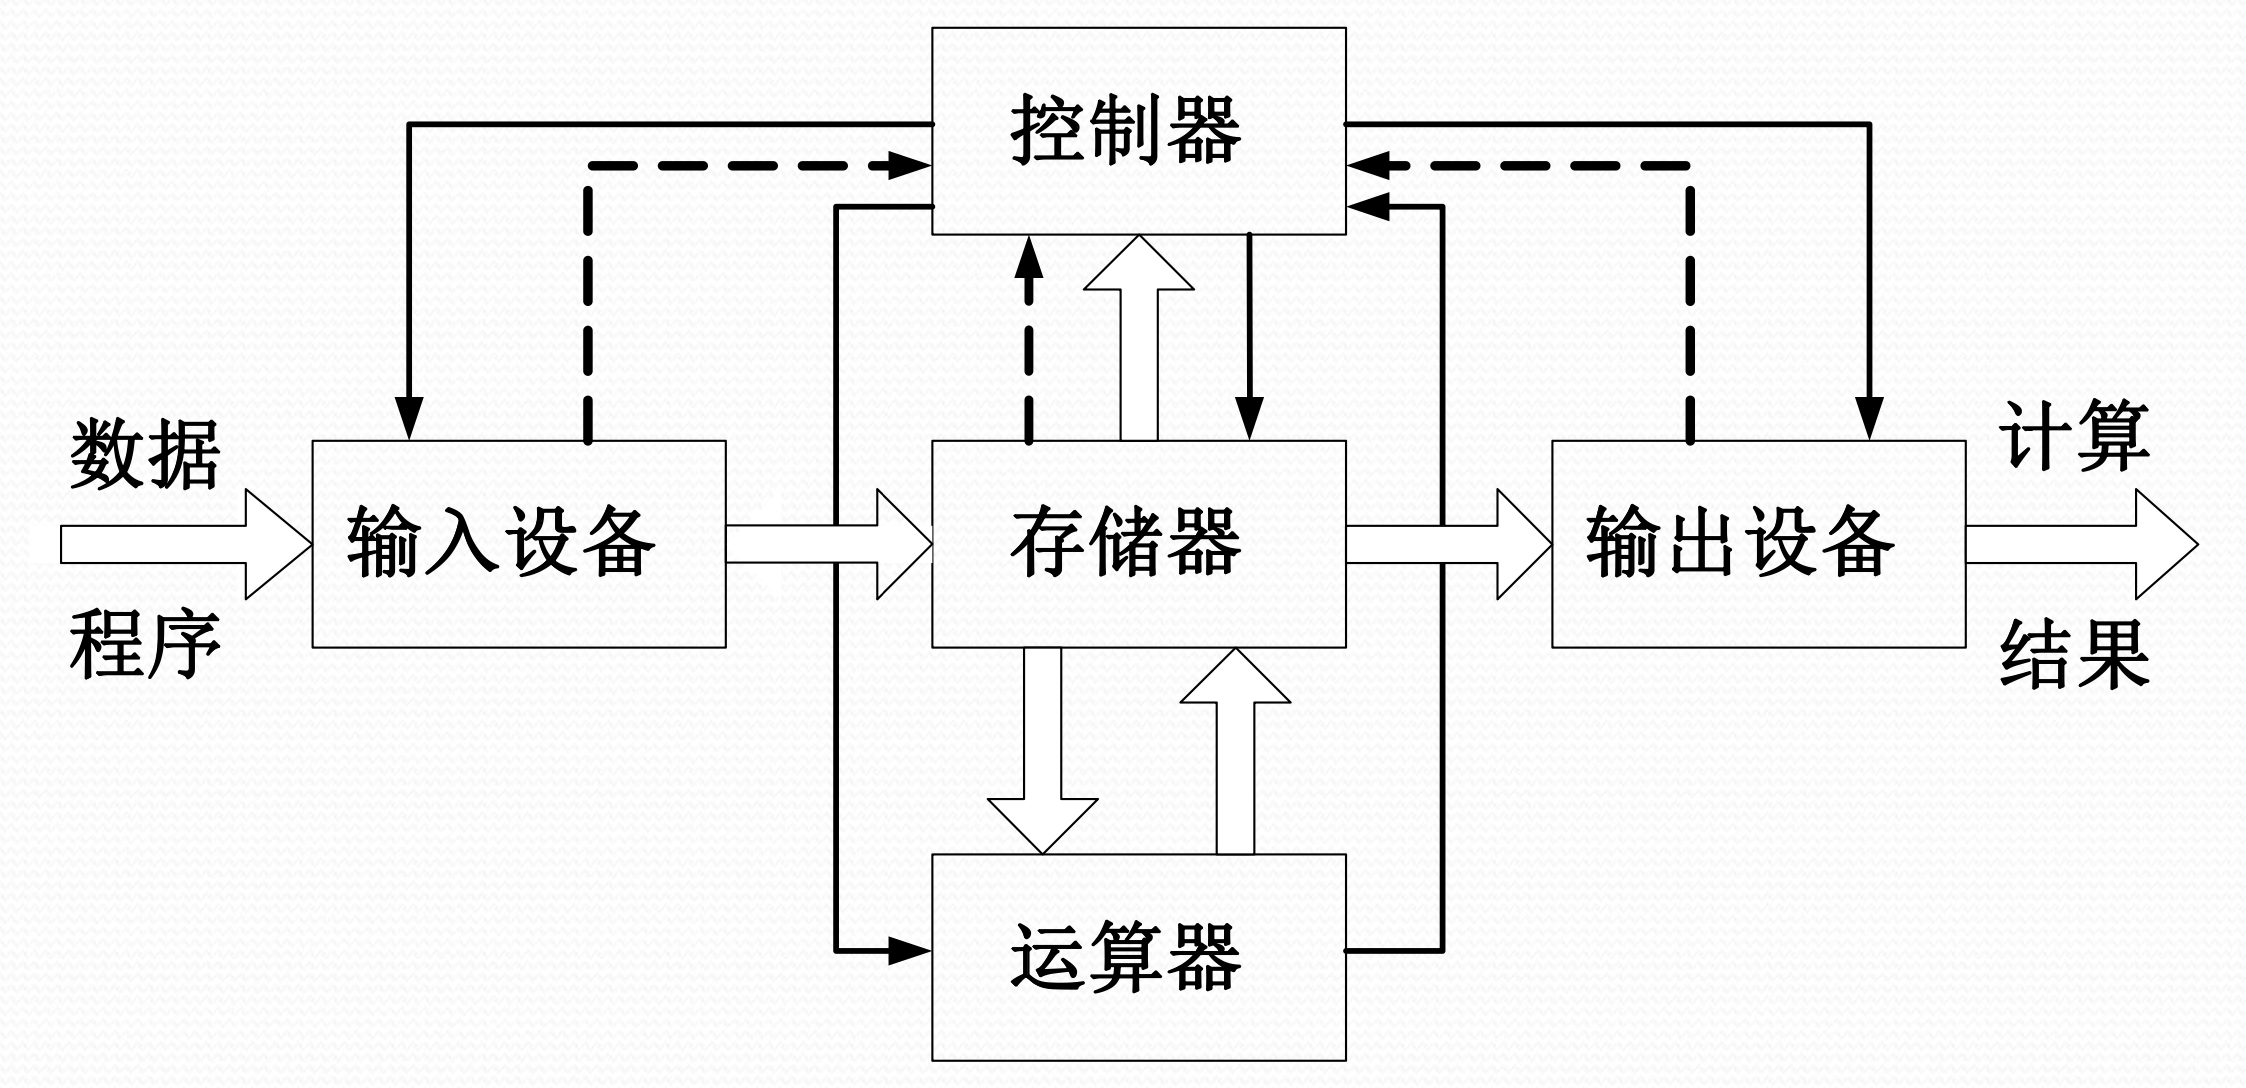
\includegraphics[width=0.6\textwidth]{img/1.1.2.2}
	\end{figure}


	\subsubsection{计算机总线与网络总线}
	\begin{itemize}
		\item 总线是计算机各种功能部件之间传送信息的公共通信干线
		\item 按照所传输的信息种类,总线可分为控制线、数据线和地址线
		\item 为了提高计算机系统通信的效率,计算机总线的设计是分级的,即计算机系统存在多类总线:
		\begin{itemize}
			\item 内部总线:用于 CPU 芯片内部连接各元件
			\item 系统总线:用于连接 CPU、存储器和各种 I/O 模块等主要部件
			\begin{itemize}
				\item PCI(外设组件互联标准)总线连接了小型计算机系统接口(SCSI)设备、局域网(LAN)设备和图形设备等块设备
				\item E(ISA)(拓展(工业标准结构))总线连接串行口、并行口、鼠标、键盘等字符型的慢速设备
			\end{itemize}
			\item 通信总线:用于计算机系统之间通信
		\end{itemize}
	\end{itemize}
	\begin{figure}[H]
		\centering
		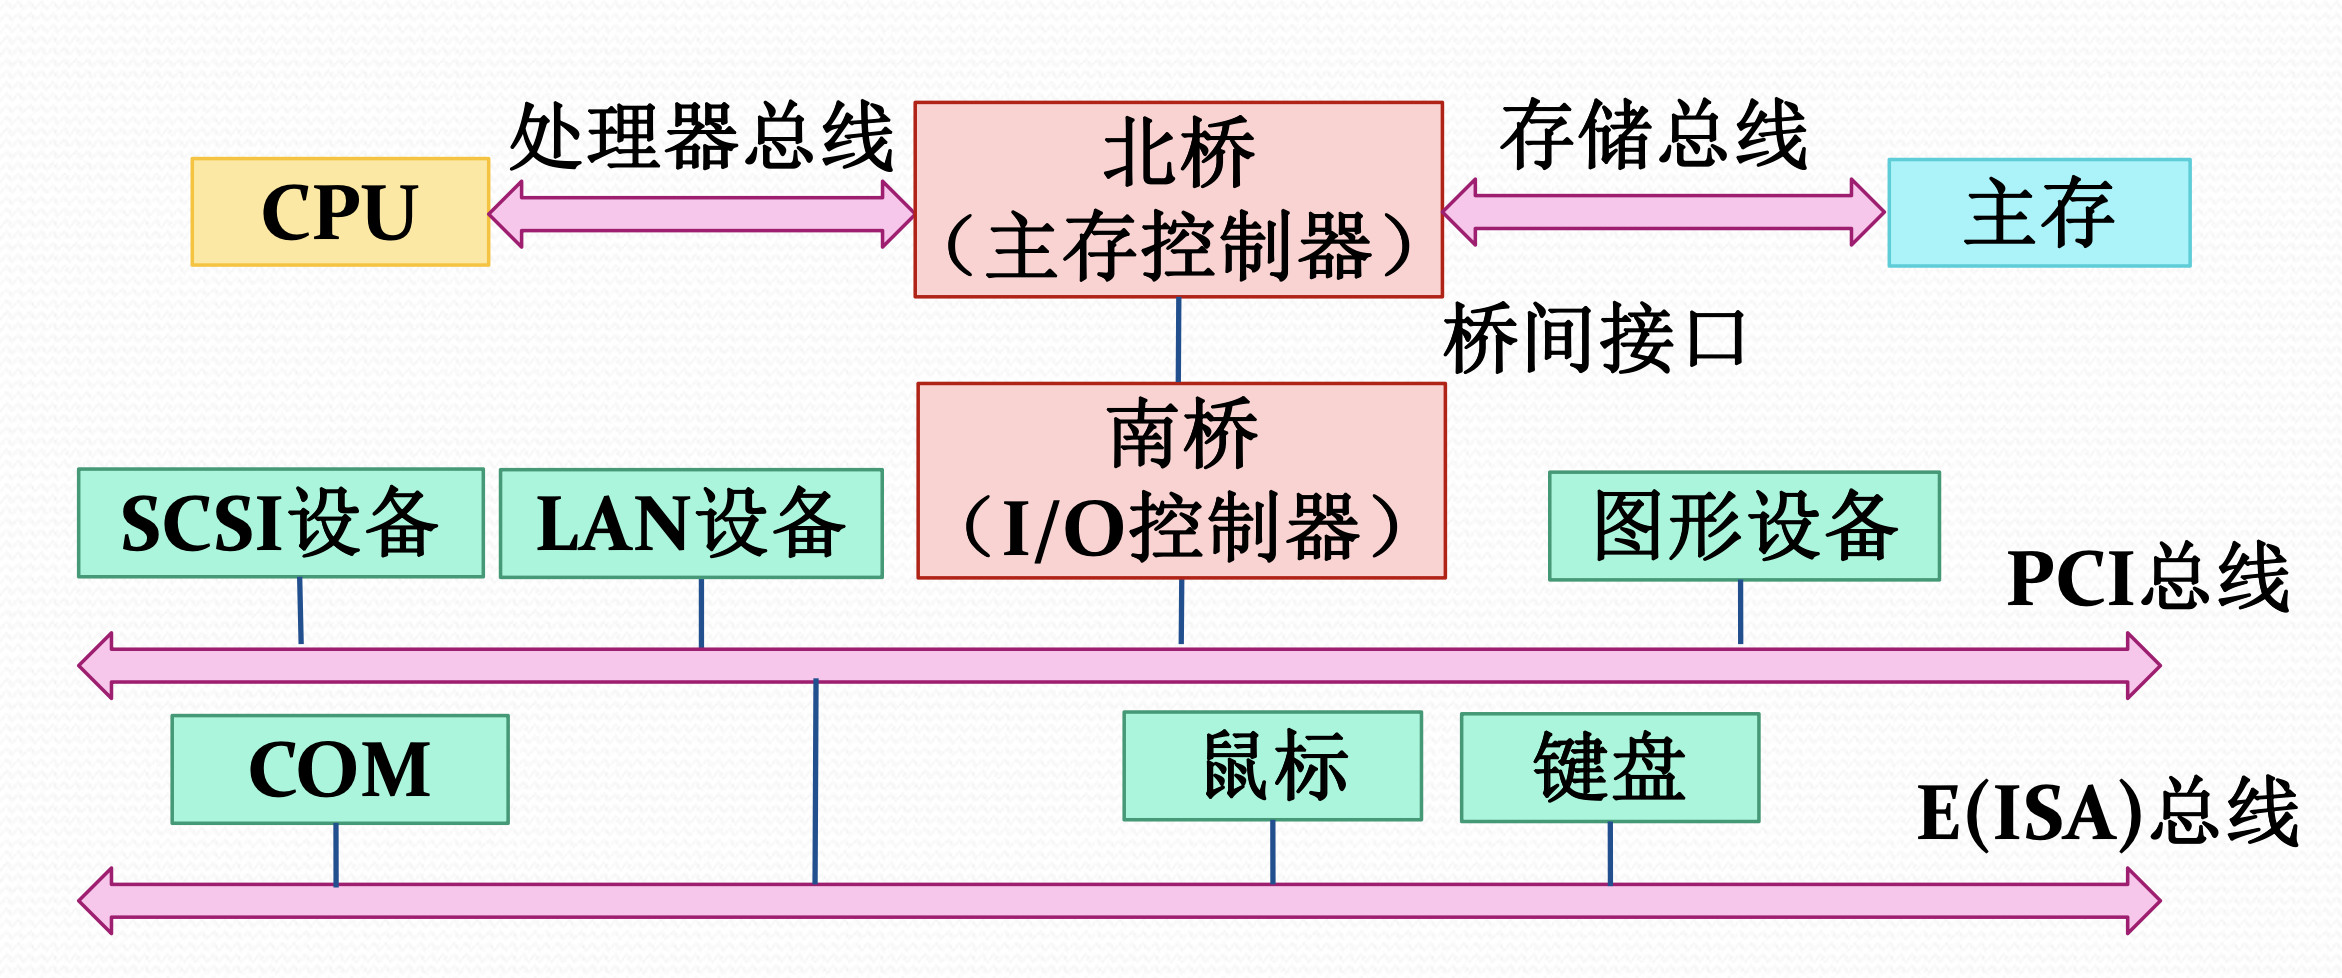
\includegraphics[width=0.7\textwidth]{img/1.1.2.3}
	\end{figure}


	\subsubsection{中央处理器}
	中央处理器是计算机的运算核心和控制核心,主要包括:
	\begin{itemize}
		\item 运算逻辑部件:一个或多个运算器
		\item 寄存器部件:包括通用寄存器、控制与状态寄存器,以及高速缓冲存储器
		\item 控制部件:实现各部件间联系的数据、控制及状态的内部总线;负责对指令译码、发出为完成每条指令所要执行操作的控制信号、实现数据传输等功能的部件
	\end{itemize}


	\subsubsection{处理器与寄存器}
	\begin{figure}[H]
		\centering
		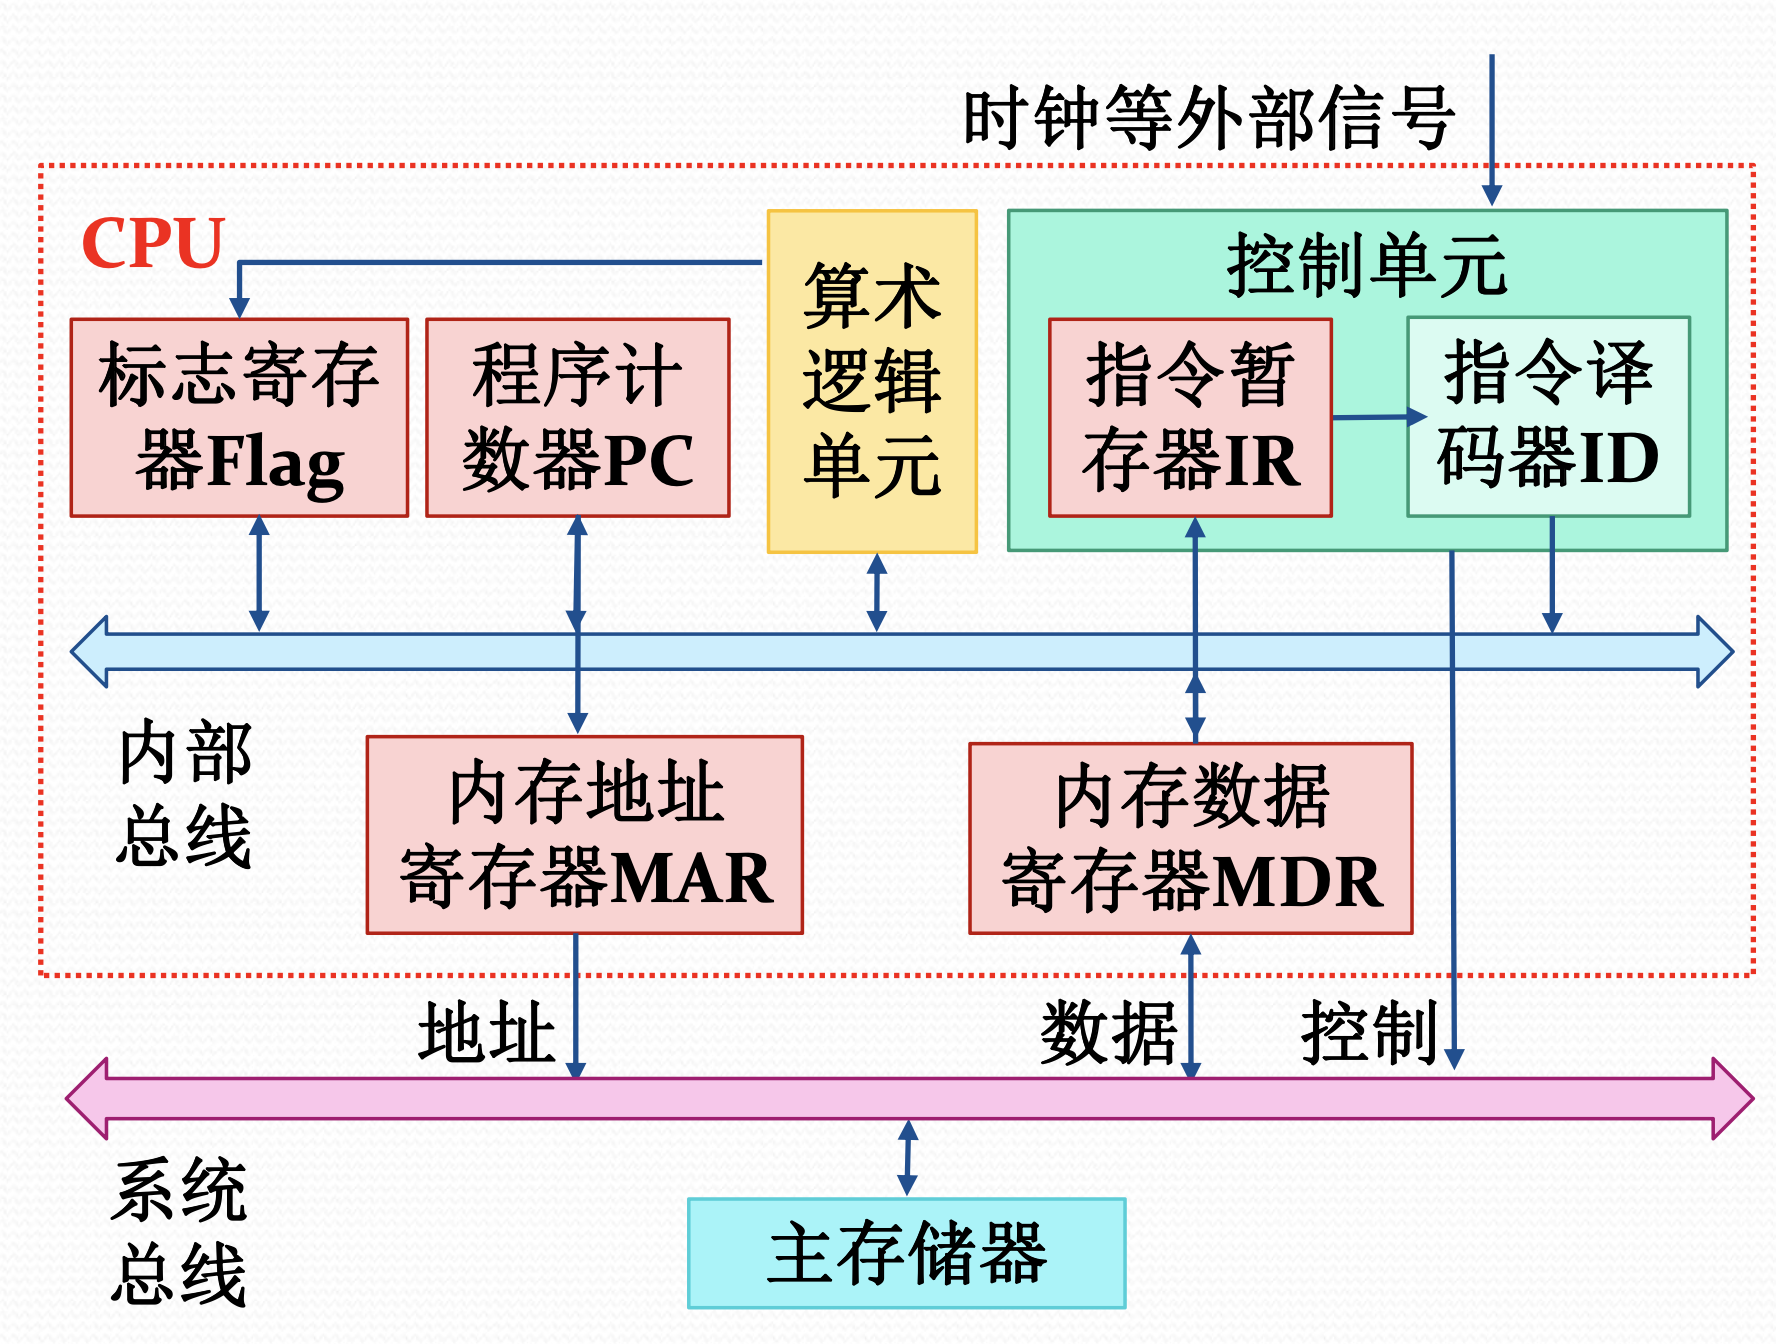
\includegraphics[width=0.65\textwidth]{img/1.1.2.5}
	\end{figure}
	上图中相比通用计算机系统缺少通用寄存器、cache 和 IOAR/IODR

	
	\subsubsection{存储器}
	存储器的组织层次如下图所示,其中主存及以上都是易失型设备
	\begin{figure}[H]
		\centering
		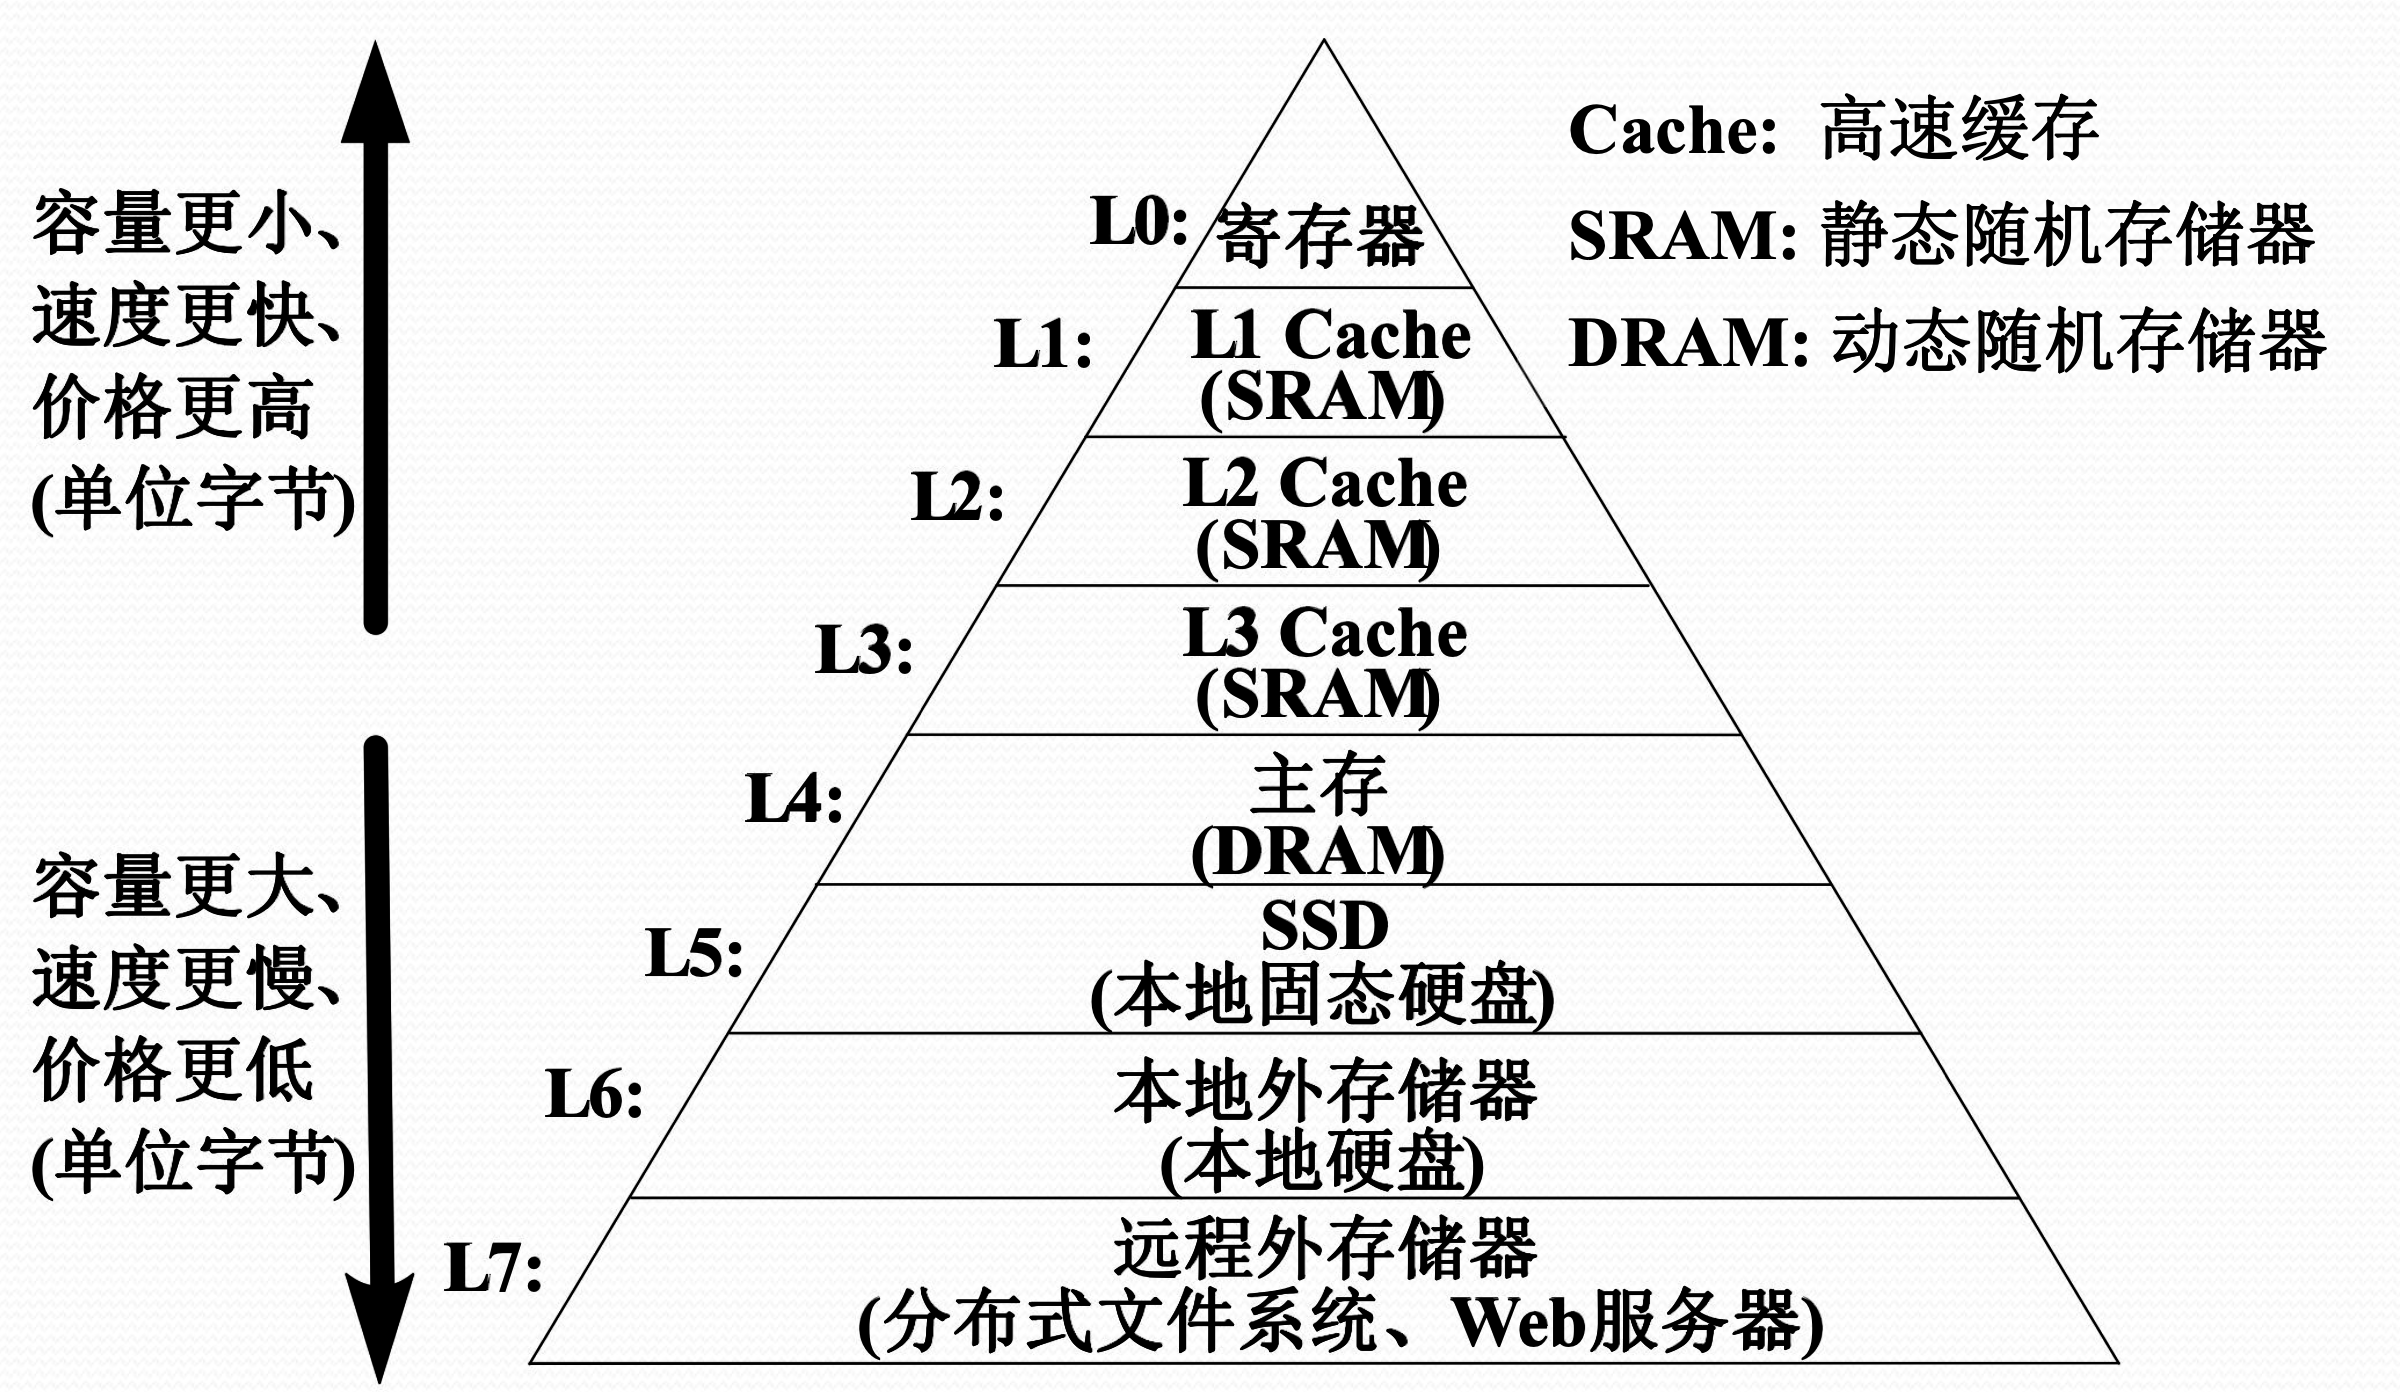
\includegraphics[width=0.6\textwidth]{img/1.1.2.6}
	\end{figure}
	

	\subsubsection{外围设备}
	计算机系统的外围设备包括输入设备、输出设备、存储设备和机机通信设备

	计算机系统需要对外围的输入/输出进行控制,控制方式主要包括:
	\begin{itemize}
		\item 轮询:CPU 忙式控制输入/输出,实现外设与主存的数据交换
		\item 中断:CPU 启动外围设备进行输入/输出;外围设备输入/输出结束后,通过中断来请求 CPU 完成后续操作;CPU 再控制外围设备与主存进行数据交换
		\item 直接存储器访问(DMA):CPU 启动 DMA 后,DMA 就可以独立地进行主存数据交换,待数据交换结束后再中断 CPU 进行后续处理
	\end{itemize}


	\subsection{计算机软件系统}
	\subsubsection{计算机软件系统的组成}
	计算机软件系统包括系统软件、支撑软件和应用软件三大组成部分
	\begin{itemize}
		\item 系统软件
		\begin{itemize}
			\item 操作系统:实施对各种软硬件资源的管理控制
			\item 应用程序:为方便用户所设,如文本编辑等
			\item 语言处理程序:把用汇编语言/高级语言编写的程序,翻译成可执行的机器语言程序
			\item 数据库管理系统
		\end{itemize}
		\item 支撑软件:支持用户使用计算机的环境,提供开发工具,也可以认为是系统软件的一部分
		\begin{itemize}
			\item 接口软件
			\item 工具软件
			\item 环境数据库等
		\end{itemize}
		\item 应用软件:用户按其需要自行编写的专用程序
	\end{itemize}


	\subsubsection{软件扩充计算机系统功能}
	\begin{itemize}
		\item 计算机硬件系统:机器指令
		\item 操作系统与实用软件:扩展机器指令,系统调用、操作系统与应用软件
		\item 数据库语言:数据库管理系统,可以不再对流进行处理,而是处理对象式和关系式
		\item 语言处理系统:高级语言,变向对目标进行解决
		\item 支撑软件:使用软件工程工具
	\end{itemize}
	\begin{figure}[H]
		\centering
		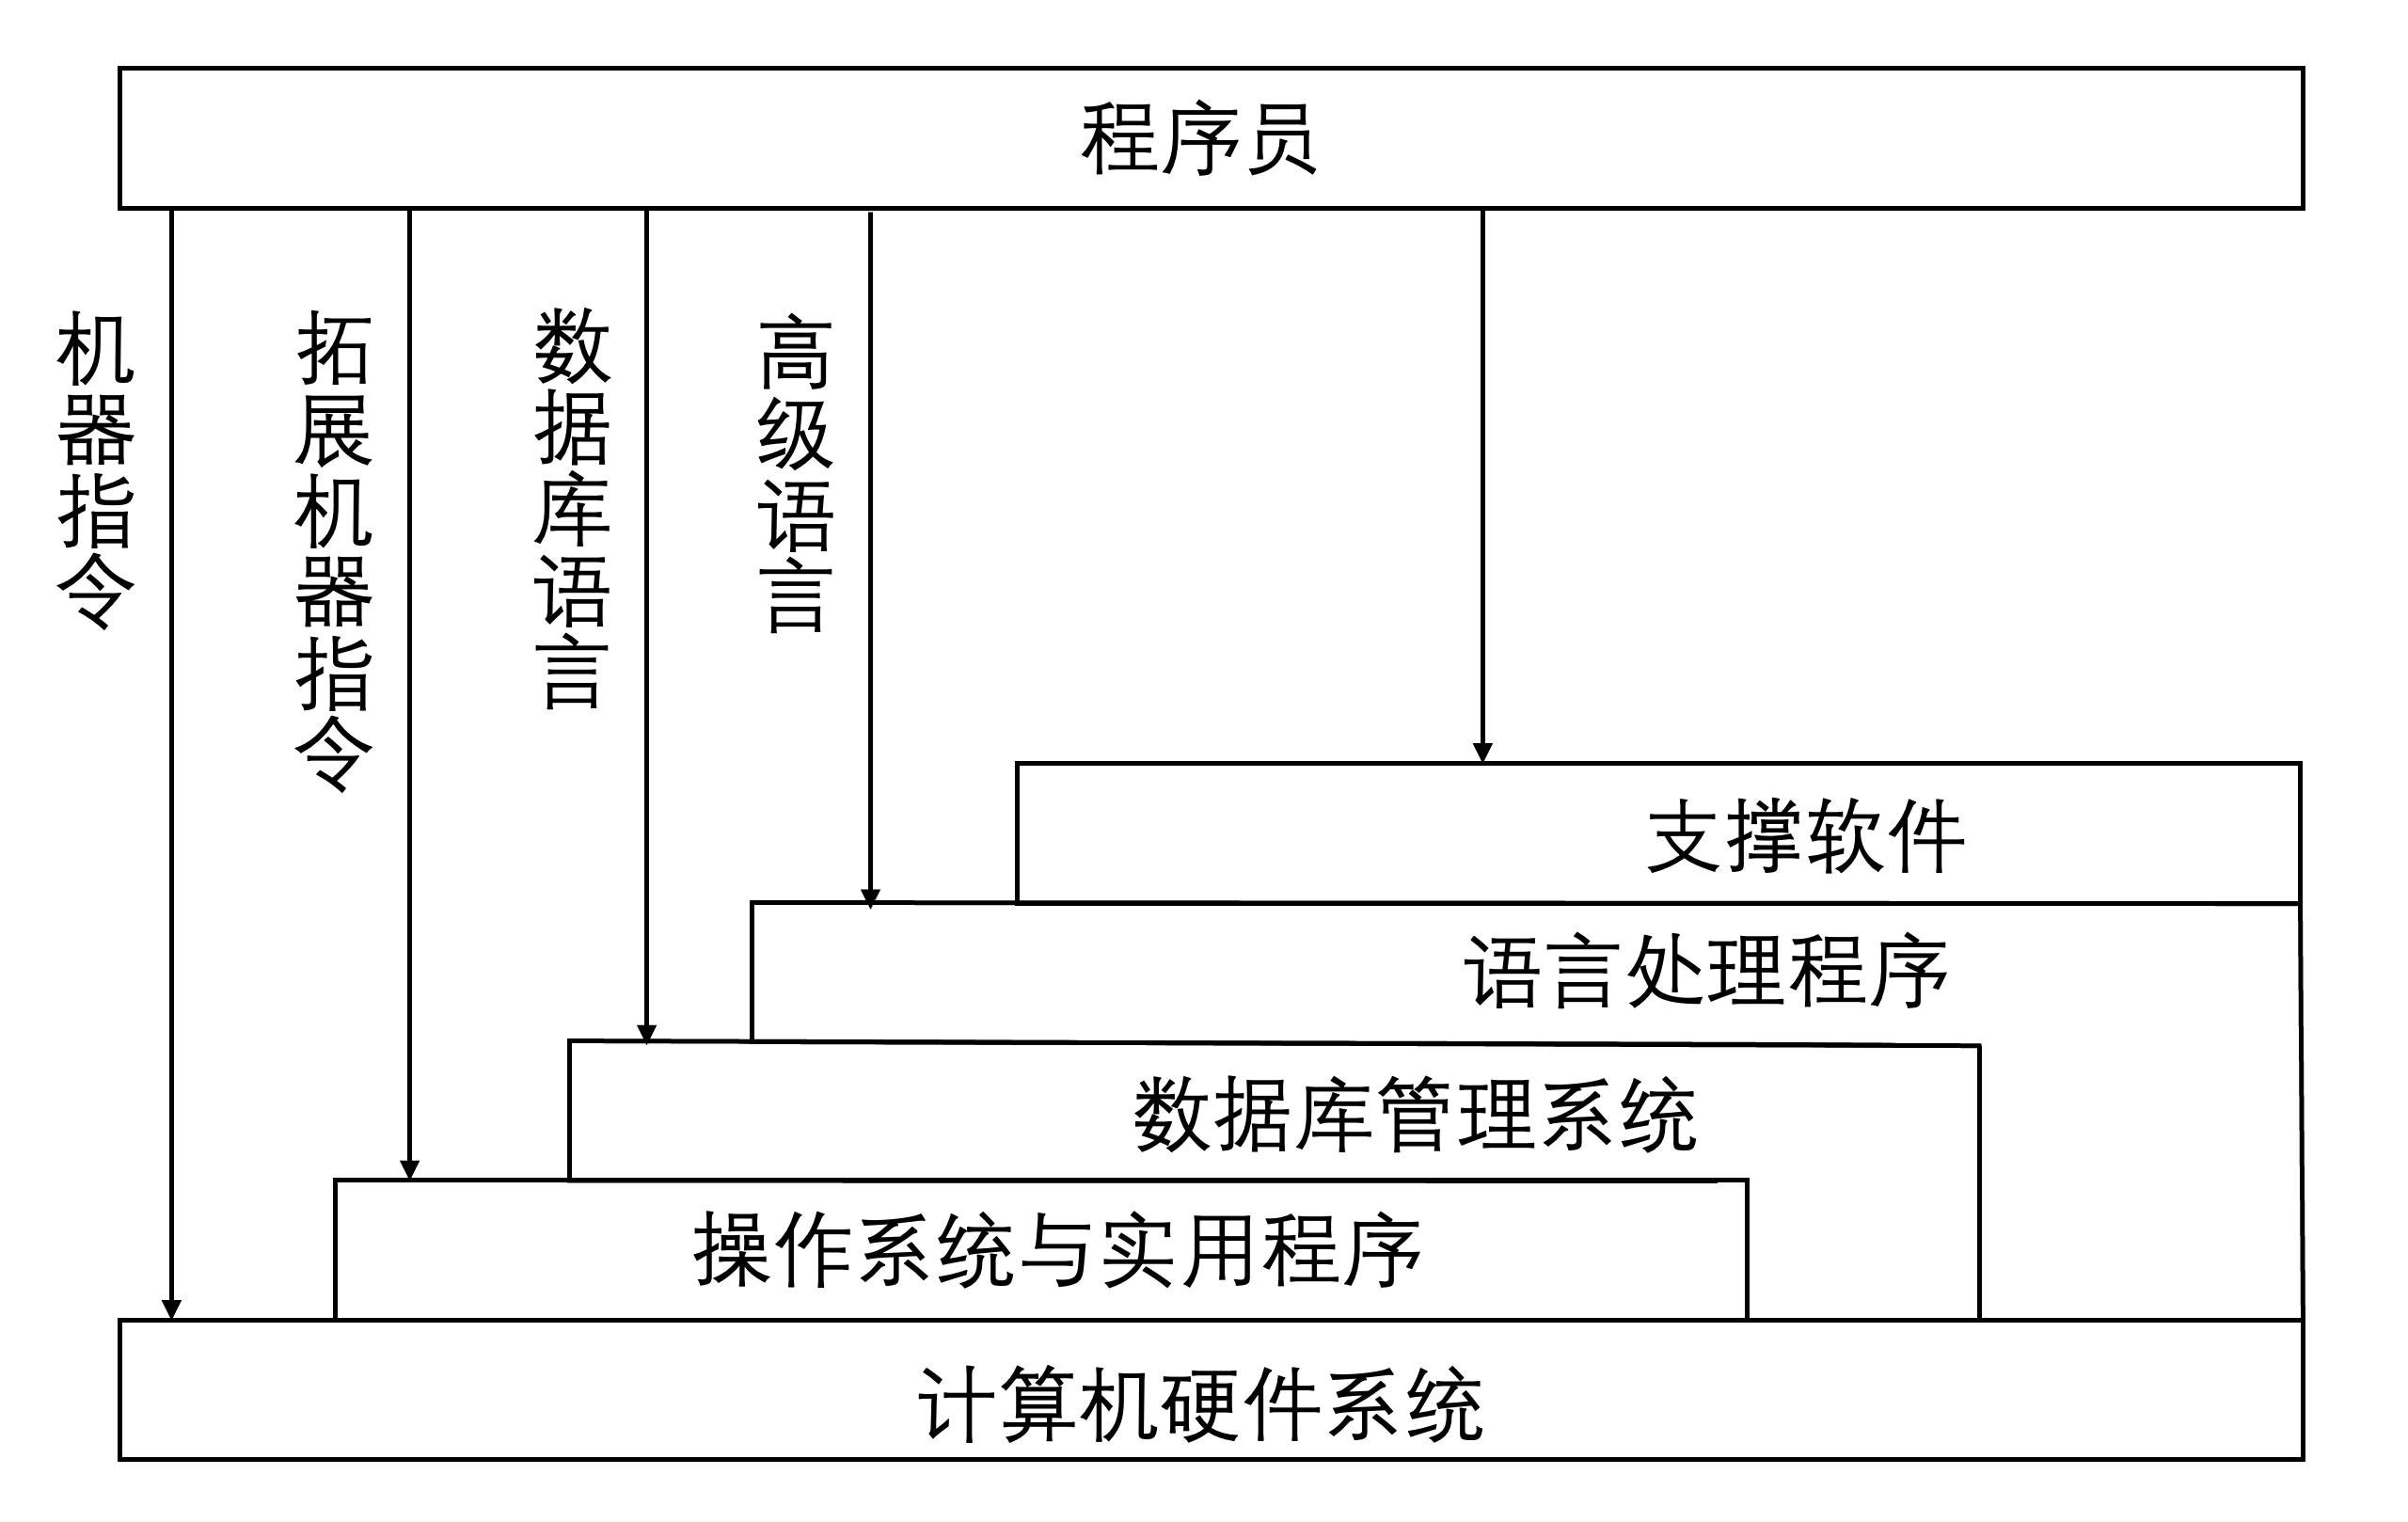
\includegraphics[width=0.6\textwidth]{img/1.1.3.2}
	\end{figure}
	软件开发的不同层次:
	\begin{itemize}
		\item 计算机硬件系统:机器语言
		\item 操作系统之资源管理:机器语言 $+$ 广义指令(扩充了硬件资源管理)
		\item 操作系统之文件系统:机器语言 $+$ 系统调用(扩充了信息资源管理)
		\item 数据库管理系统:$+$ 数据库语言(扩充了功能更强的信息资源管理)
		\item 语言处理程序:面向问题的语言
	\end{itemize}

	
	\subsubsection{计算机程序的解译执行过程}
	\begin{figure}[H]
		\centering
		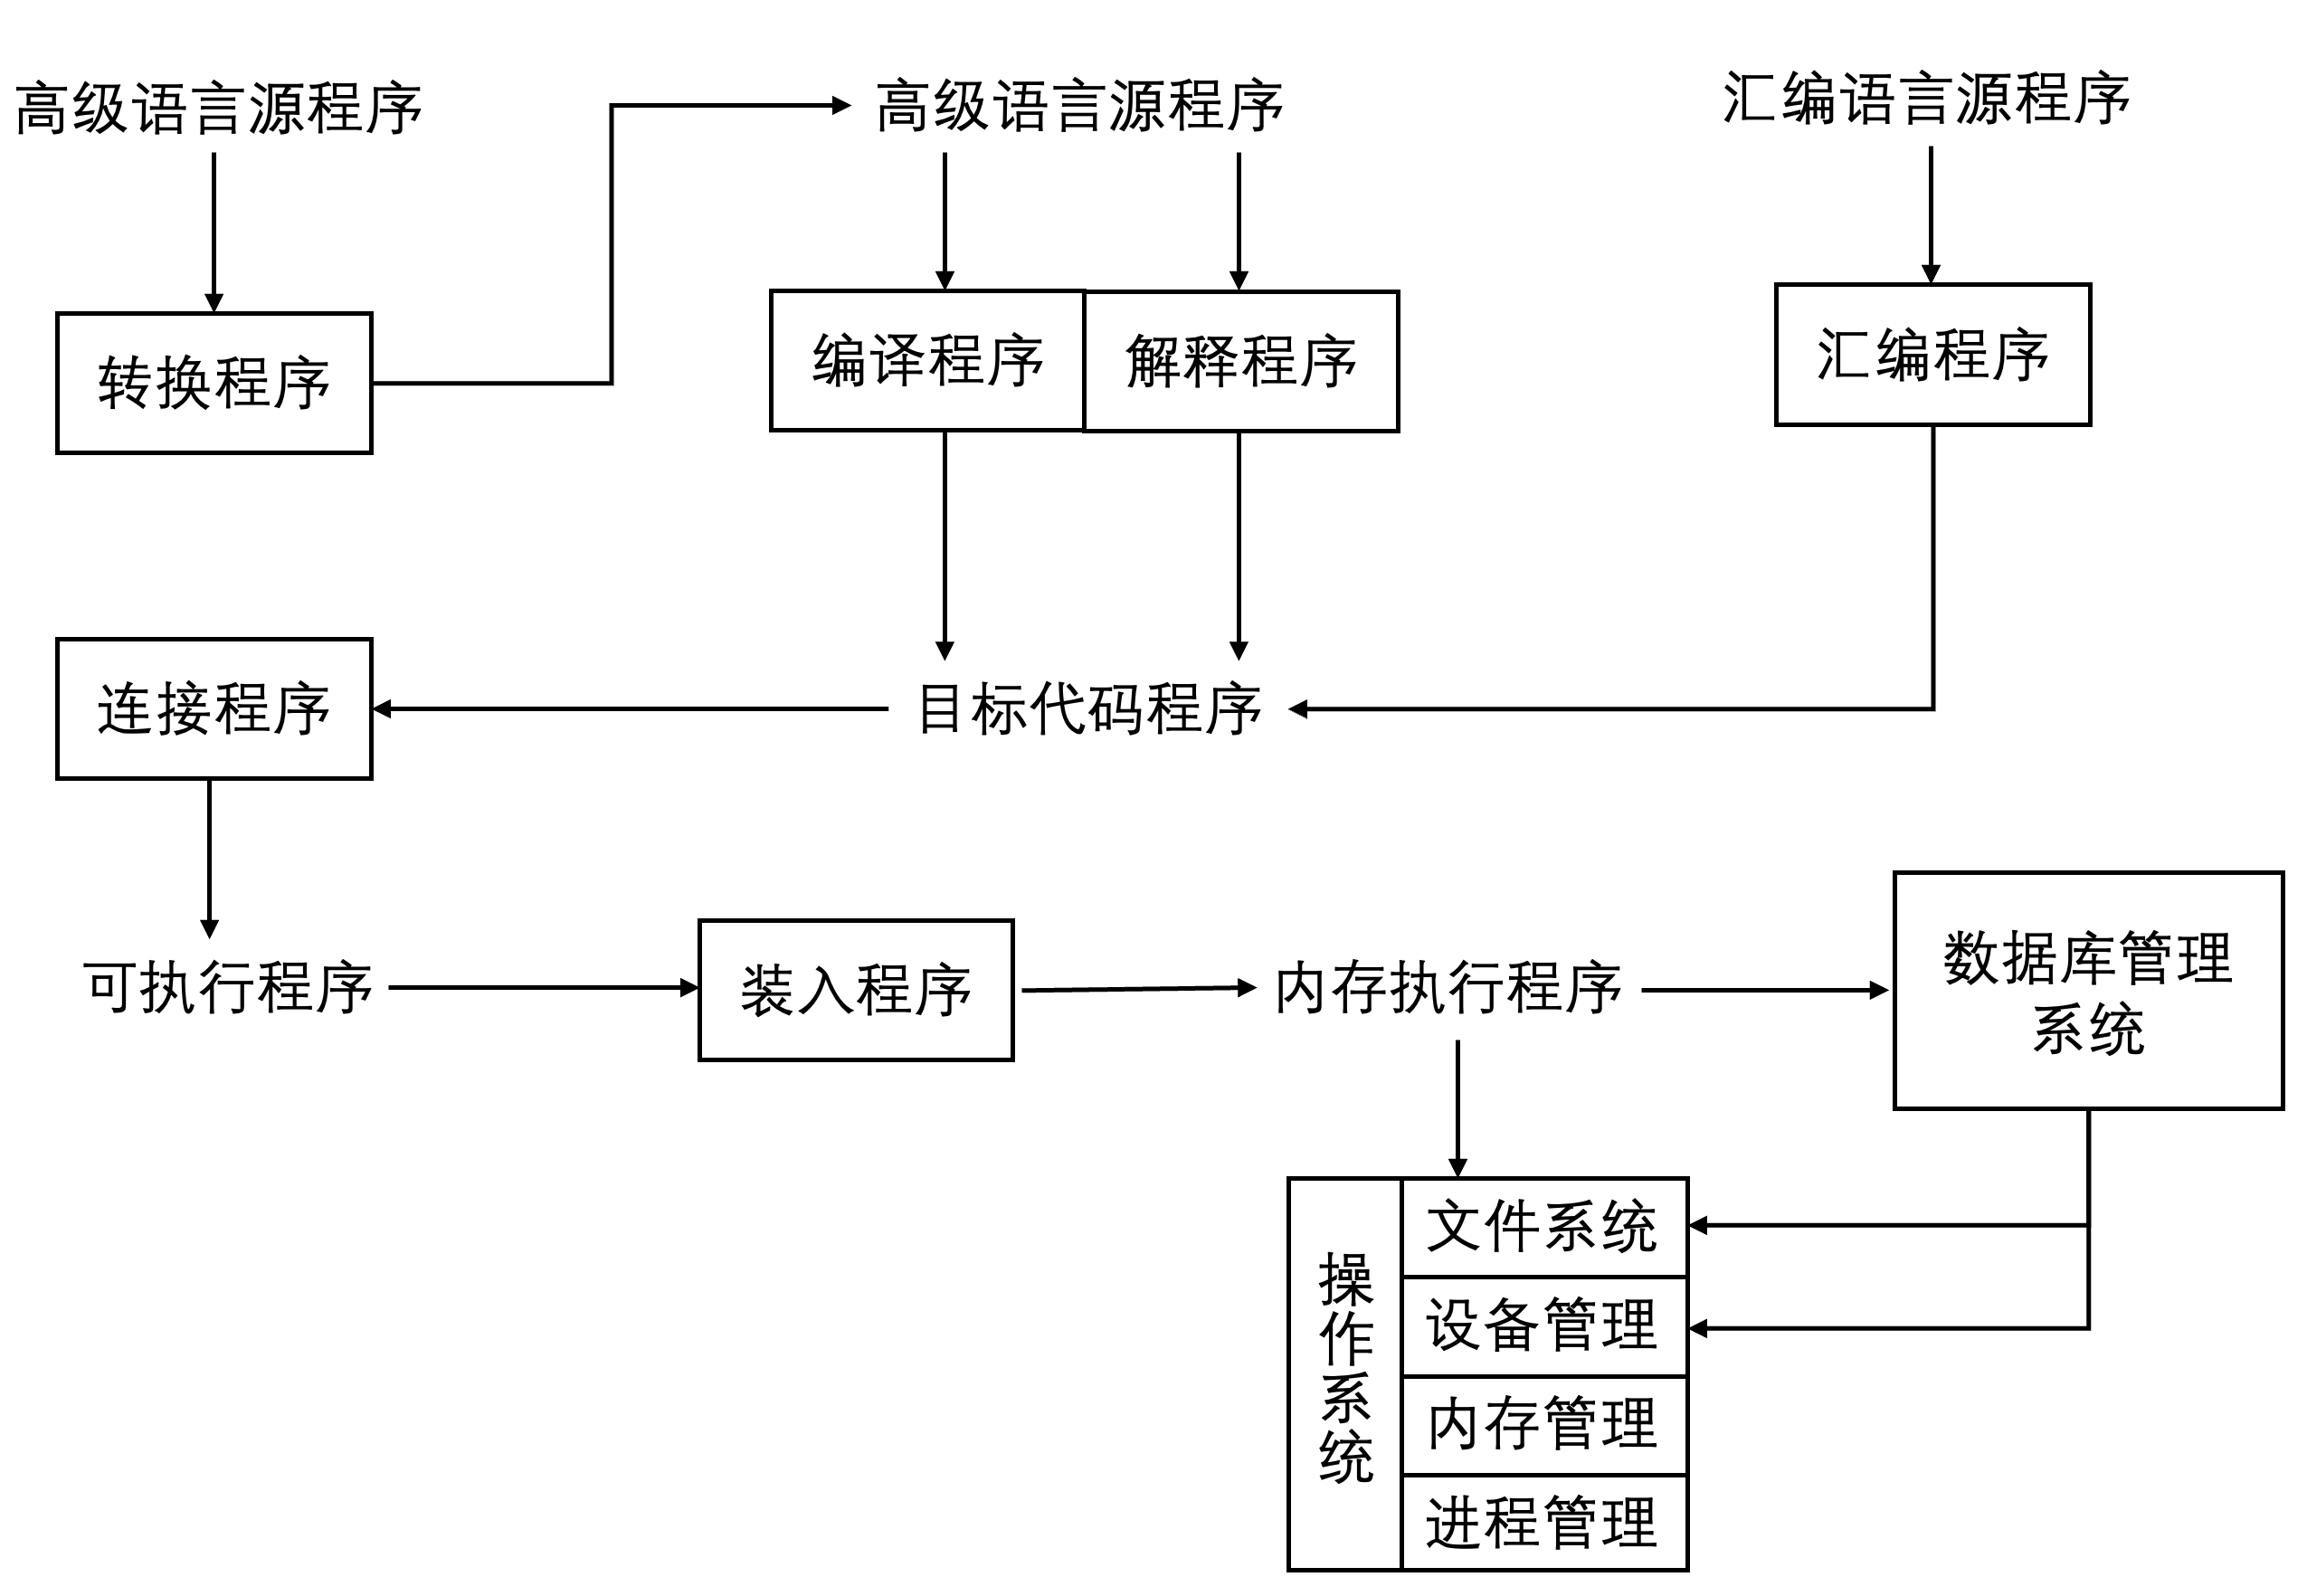
\includegraphics[width=0.8\textwidth]{img/1.1.3.3}
	\end{figure}
	上图给出的是裸机上计算机程序的解译执行过程,现代计算机系统在实现时往往是基于虚拟机的,即基于一汇编指令集合提供计算功能。在这种情况下,目标代码变成了单纯的汇编指令,而汇编程序的功能则变成了程序优化



	\section{计算机操作系统}
	\subsection{计算机操作系统的发展}
	\subsubsection{计算机的手工操作}
	最初的计算机操作控制方式可以表示为开关表示、按钮控制、亮灯显示
	\begin{figure}[H]
		\centering
		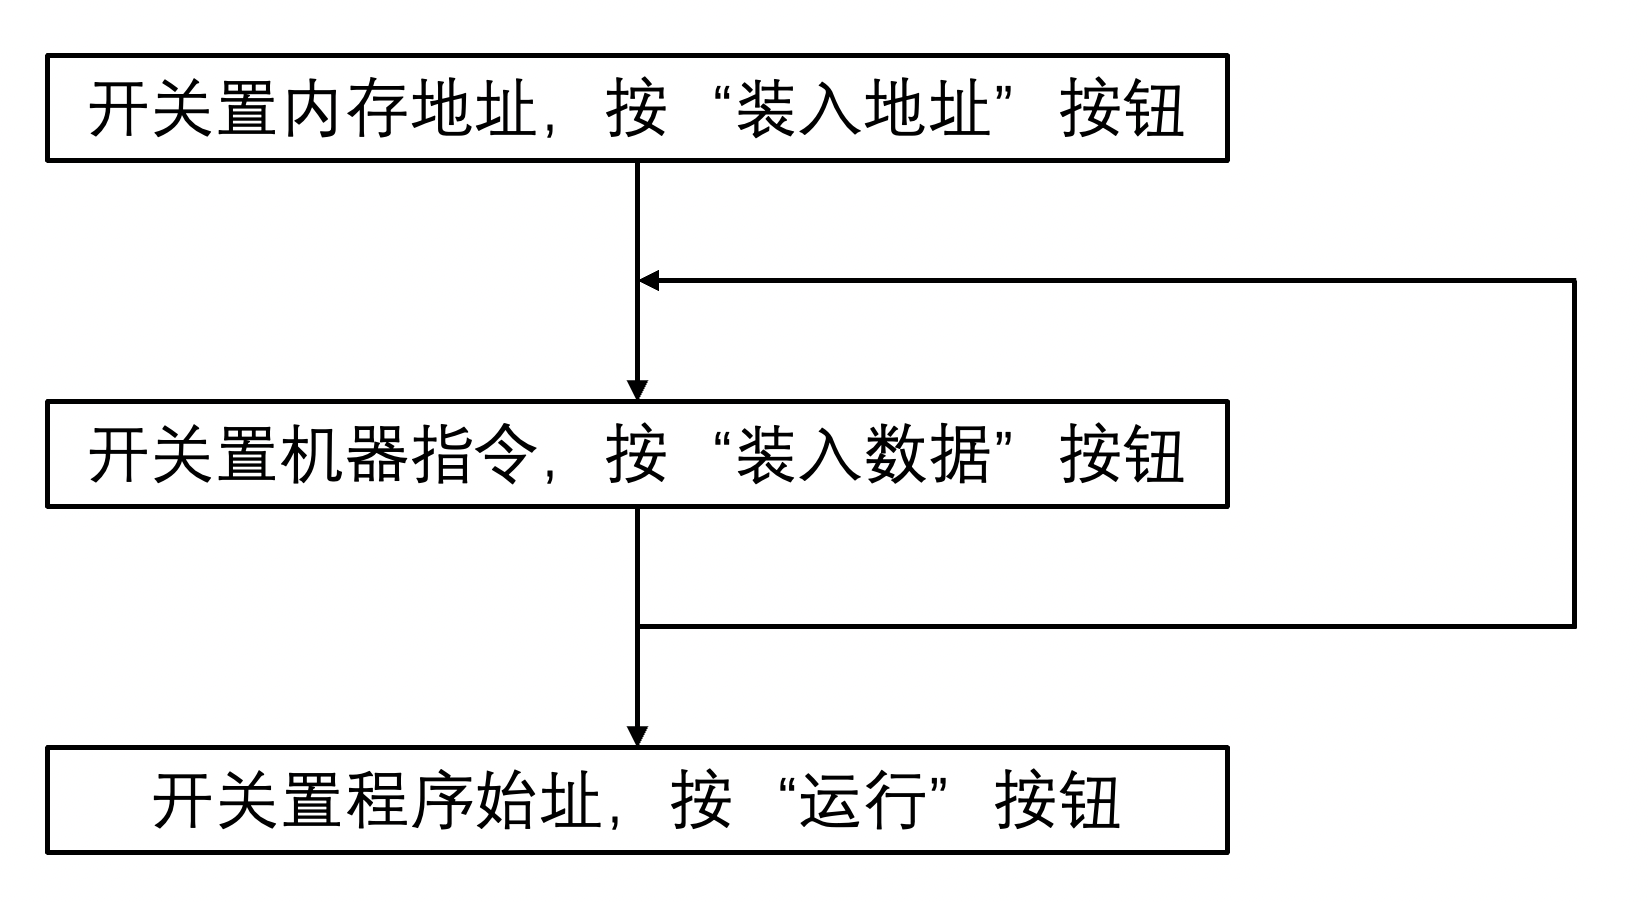
\includegraphics[width=0.5\textwidth]{img/1.2.1.1}
	\end{figure}


	\subsubsection{装入程序的引进}
	\begin{itemize}
		\item 引入卡片和纸带描述程序指令与数据
		\item 引入装入程序
		\begin{itemize}
			\item 自动化执行程序装入,必要时进行地址转换
			\item 通常存放在 ROM 中
		\end{itemize}
	\end{itemize}
	\begin{figure}[H]
		\centering
		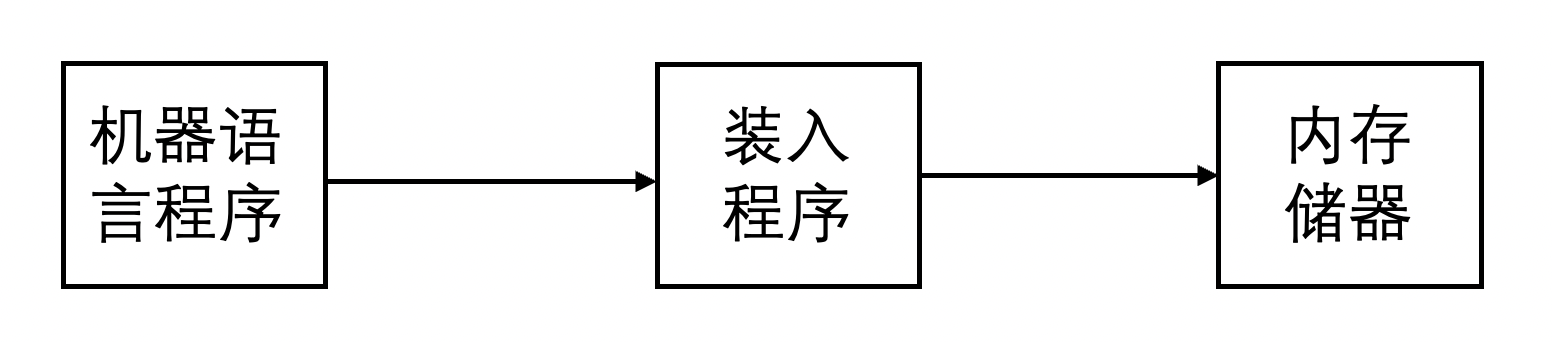
\includegraphics[width=0.5\textwidth]{img/1.2.1.2}
	\end{figure}


	\subsubsection{引入汇编语言后的计算机控制}
	\begin{figure}[H]
		\centering
		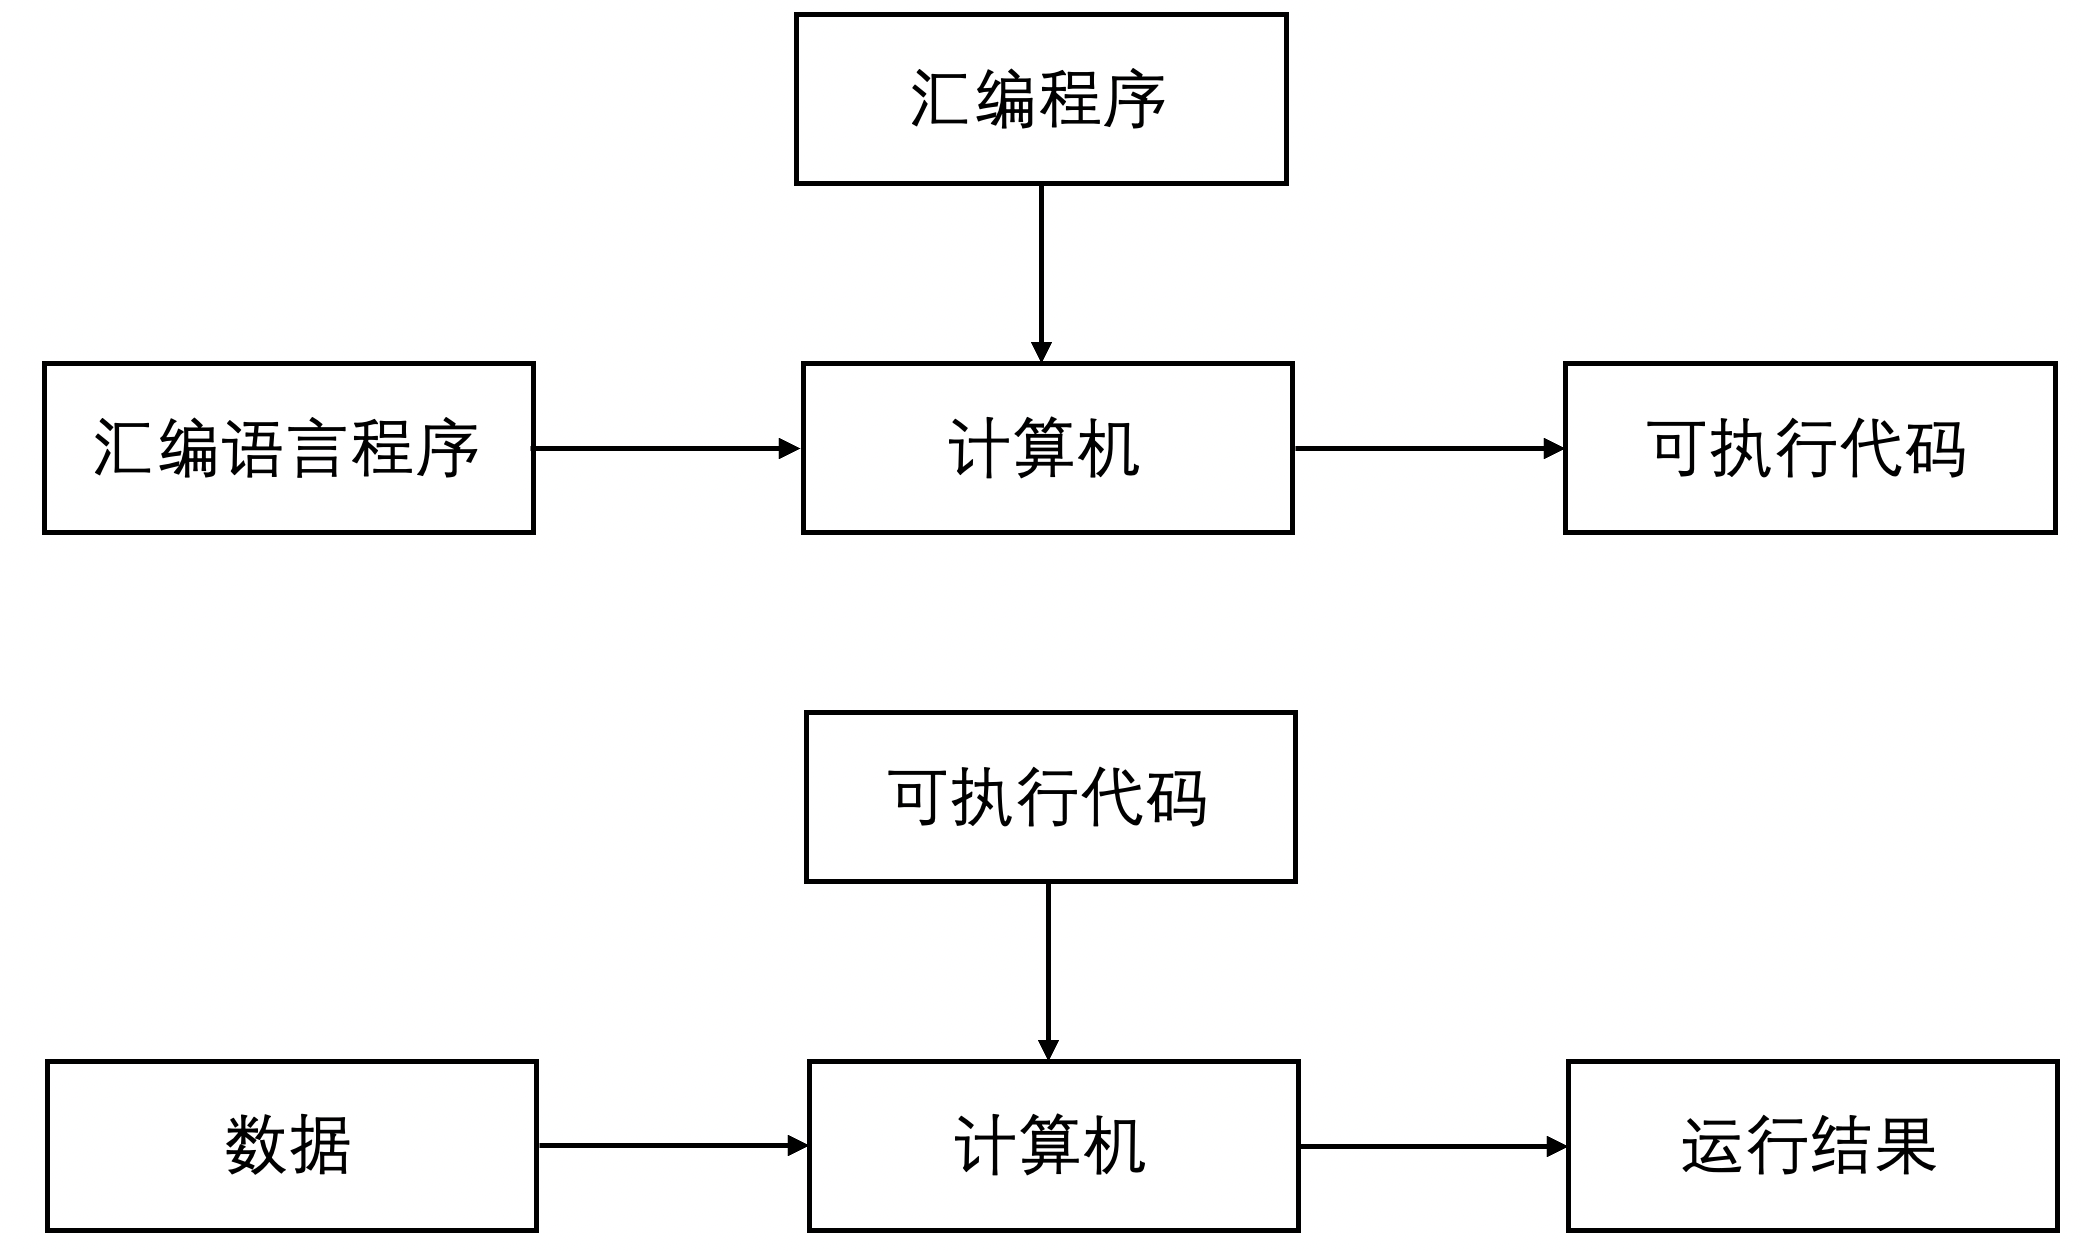
\includegraphics[width=0.6\textwidth]{img/1.2.1.3}
	\end{figure}


	\subsubsection{引入高级语言后的计算机控制}
	\begin{figure}[H]
		\centering
		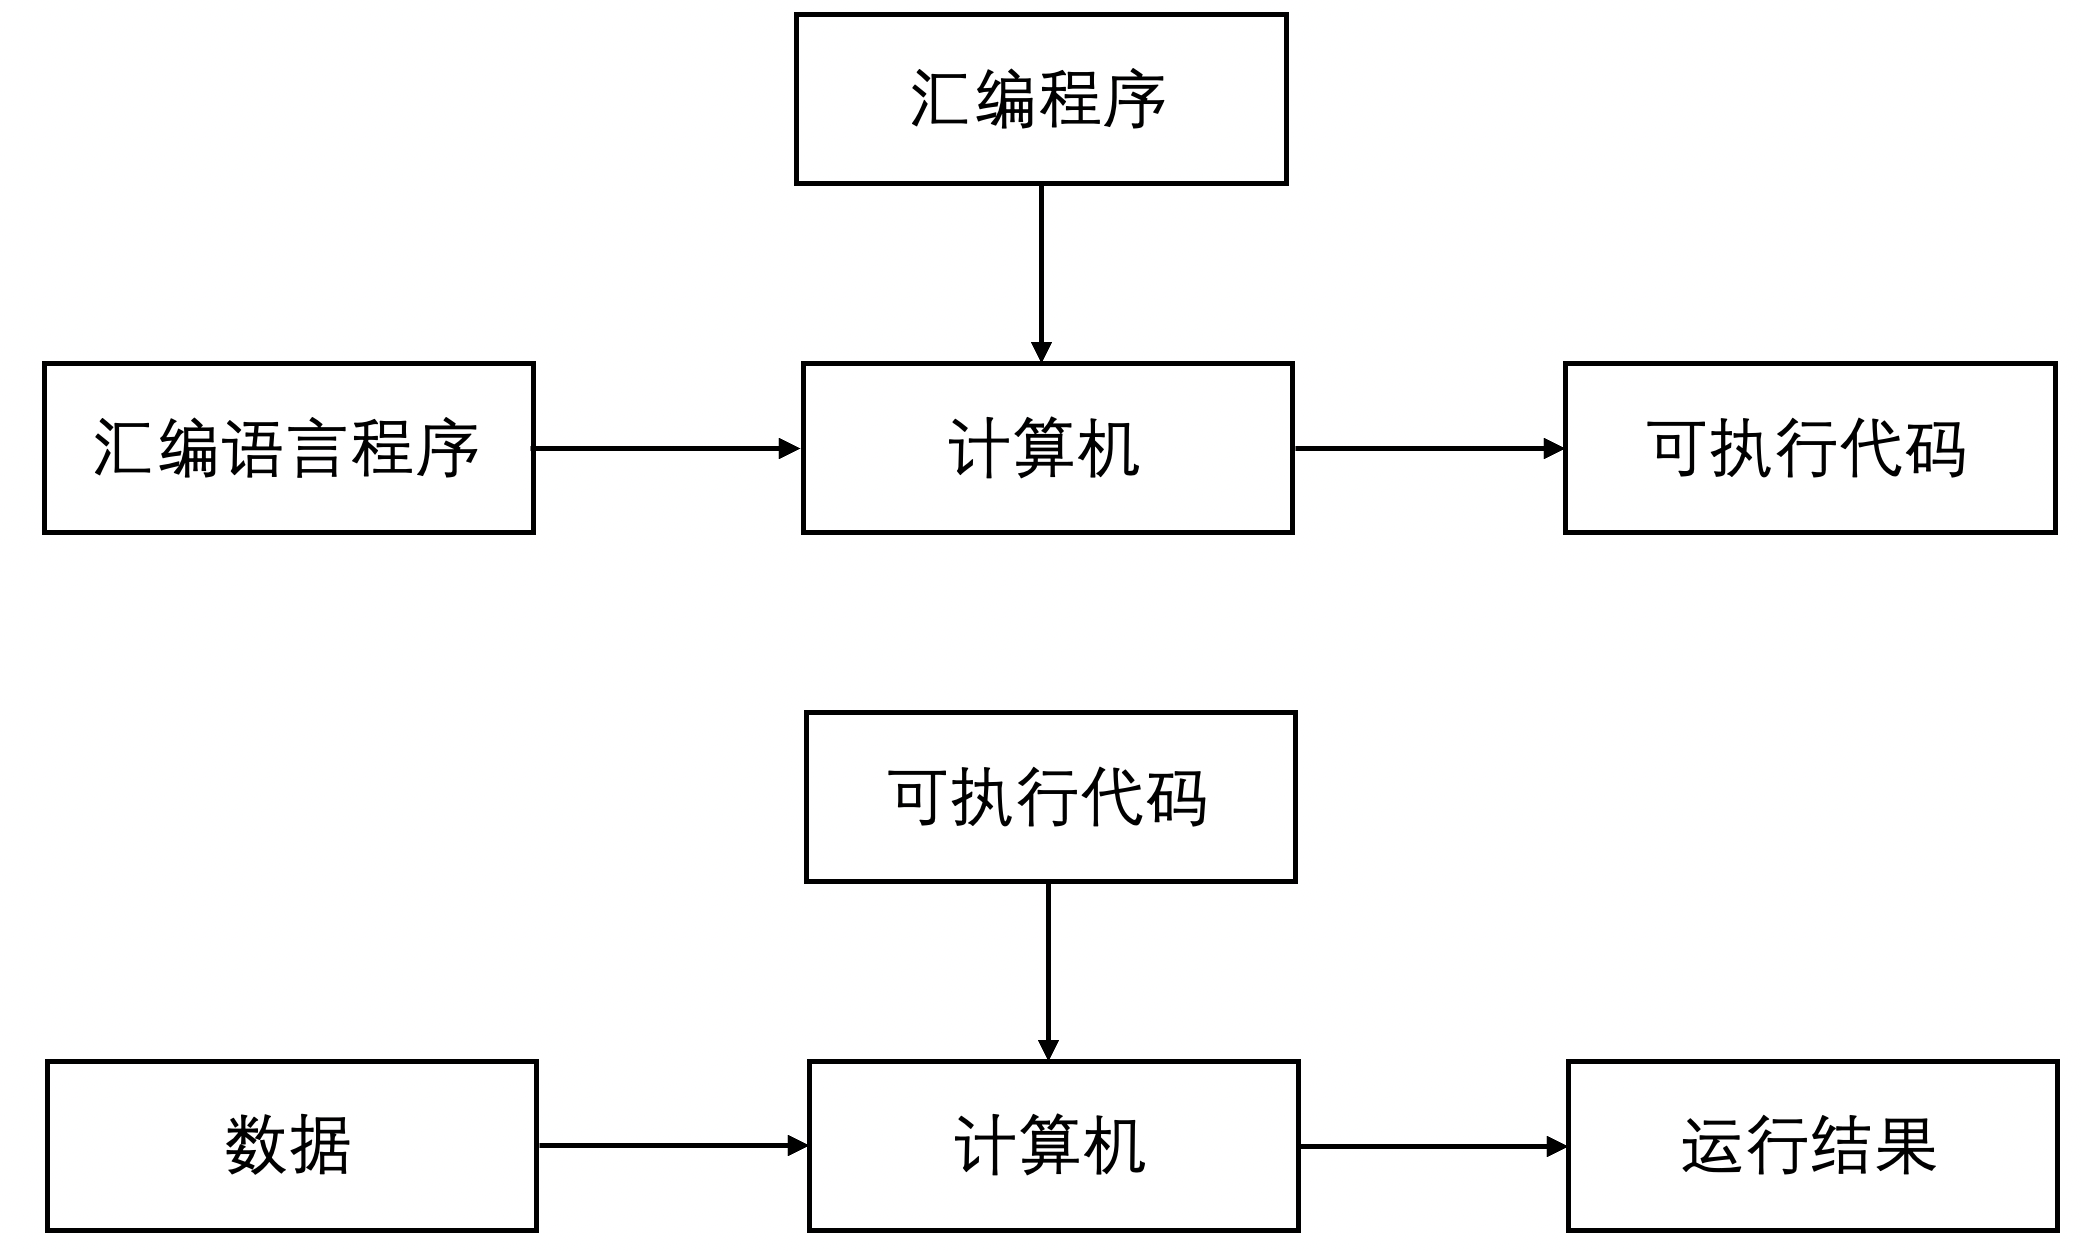
\includegraphics[width=0.6\textwidth]{img/1.2.1.3}
	\end{figure}


	\subsubsection{简单批处理系统的操作控制}
	\begin{itemize}
		\item 简单批处理系统的处理过程
		\item 这一方式明显缩短了手工操作的时间,提高了计算机系统利用率
		\item 这一阶段,磁带的出现,使得卡片与纸带等机械输入方式得以进一步提高
		\item 简单批处理系统本质上是一种半自动化的操作方式,不算操作系统
		\begin{itemize}
			\item 解决了手工操作和计算机机械操作不匹配的矛盾
			\item 没有解决了手工操作与中央处理器电子操作速度不匹配的矛盾
			\item 进一步减少了慢速外设的影响
		\end{itemize}
		\item 简单批处理系统的解决方案是允许多道程序同时运行,但是没有达到真正的多道程序设计
	\end{itemize}


	\subsubsection{操作系统与自动化操作控制}
	\begin{itemize}
		\item 电子计算速度与机械 I/O 速度的矛盾:你在输,我在等
		\item 在程序执行过程中能否同时输入作业重叠时间
		\begin{itemize}
			\item 需要多道程序同时执行
			\item 程序切换需要高速的外存储设备
		\end{itemize}
		\item 磁盘设备出现:计算机操作系统浓墨登场,实现了计算机系统的自动化控制
	\end{itemize}


	\subsection{操作系统及其分类}
	\subsubsection{操作系统}
	\textbf{操作系统是计算机系统最基础的系统软件,管理软硬件资源、控制程序执行,改善人机界面,提供各种服务,合理组织计算机工作流程,为用户使用计算机提供良好运行环境。}
	\begin{itemize}
		\item 计算机系统最基础的系统软件:处于硬件之上(最接近硬件)的系统软件
		\item 管理软硬件资源:
		\begin{itemize}
			\item 管理硬件资源,首先进行抽象,提供系统调用和中断等服务给上层资源使用
			\item 管理软件资源,管理文件抽象的数据资源以及在操作系统环境下可能被启动运行的应用程序,并创建成进程,然后再为进程分配相应的资源,包括 CPU 资源、处理器资源、外设资源和程序运行中的文件系统需要的资源。也可以映射为三个基本抽象
		\end{itemize}
		\item 控制程序的执行:在操作系统环境下,加入的软件系统的实体,要被创建成一些进程,并由操作系统来统管所有的进程
		\item 改善人机界面:操作系统最终是呈现给终端用户使用,必须改善用户界面,方便人群使用。由于操作系统定位的人群不同,则风格不同,比如服务器的命令行控制
		\item 合理组织计算机工作流程:体现资源调度和管理
		\item 为用户使用计算机提供良好运行环境
	\end{itemize}


	操作系统是方便用户、管理和控制计算机软硬件资源的系统程序集合
	\begin{itemize}
		\item 从\textbf{用户}角度看,操作系统管理计算机系统的各种资源,扩充硬件的功能,控制程序的执行
		\item 从\textbf{人机交互}角度看,操作系统是用户与机器的接口,提供良好的人机界面,方便用户使用计算机,在整个计算机系统中具有承上启下的地位
		\item 从\textbf{系统结构}角度看,操作系统是一个大型软件系统,其功能复杂,体系庞大,采用层次式、模块化的程序结构
	\end{itemize}

	操作系统是软件系统的核心,与硬件一同构成了各种软件的基础服务平台
	\begin{itemize}
		\item 服务用户:操作系统作为用户接口和公共服务程序
		\item 进程交互:操作系统作为进程执行的控制者和协调者
		\item 系统实现:操作系统作为扩展机或虚拟机
		\item 资源管理:操作系统作为资源的管理者和控制者
	\end{itemize}


	\subsection{操作系统的组成}
	\begin{table}[H]
		\centering
		\begin{tabular}{|c|l|}
			\hline
			操作系统组成的子系统 & \multicolumn{1}{c|}{描述}                                                                              \\ \hline
			进程调度子系统    & 负责管理调度进程                                                                                             \\ \hline
			进程通信子系统    & 负责进程间的通信解决方案                                                                                         \\ \hline
			内存管理子系统    & 负责管理内存与虚存                                                                                            \\ \hline
			设备管理子系统    & 负责管理我们的外围设备                                                                                          \\ \hline
			文件管理子系统    & \begin{tabular}[c]{@{}l@{}}负责管理文件信息,提供系统调用,Linux 需要考虑如何在线性的地址\\ 空间,建立非线性的层次式目录结构以实现按名存储\end{tabular} \\ \hline
			网络通信子系统    & 实现网络操作系统,涉及到分布式等                                                                                     \\ \hline
			作业控制子系统    & 提供用户操作控制计算机系统,在服务器、云计算等资源虚拟化环境下                                                                      \\ \hline
		\end{tabular}
		\end{table}


		\subsubsection{操作系统的类型}
		\paragraph{从控制方式角度看}~{}


		\begin{itemize}
			\item 多道批处理操作系统
			\begin{itemize}
				\item 采用脱机控制方式
				\item 程序员通过作业说明来描述对作业的控制方式
				\item 操作员根据说明书来成批加载作业和控制计算机系统
				\item 优点:资源利用率高,作业吞吐量大
				\item 缺点:作业周转周期长、不具备交互式计算能力,不利于程序的开发和测试
			\end{itemize}
			\item 分时操作系统:交互控制,核心是划分 CPU 的时间
			\begin{itemize}
				\item 时间片调度思想:CPU 的时间等分
				\item 在终端上进行交互式会话,具有同时性、独立性、及时性和交互性的特点
				\item 和批处理操作系统区别:追求目标、适应作业、资源利用率不同
			\end{itemize}
			\item 实时操作系统:支持分时交互,又有大量的进程处理突发任务
			\begin{itemize}
				\item 硬实时:最严格的实时操作系统
				\item 软实时:可以在某些地方不严格
			\end{itemize}
			\item 如果某个操作系统兼具批处理、分时和实时处理的全部或两种功能,则可以被称为通用操作系统
		\end{itemize}


		\paragraph{从应用领域角度看}~{}

		\begin{itemize}
			\item 服务器操作系统:并行操作系统
			\item 网络操作系统:分布式操作系统
			\item 个人机操作系统:手机操作系统
			\item 嵌入式操作系统:传感器操作系统
		\end{itemize}


		\subsubsection{操作系统的功能和特性}
		\paragraph{操作系统功能}~{}

		\begin{itemize}
			\item \textbf{处理器管理}:对处理器的管理和调度最终归结为对进程和线程的管理和调度,最大限度提高处理器利用率
			\item \textbf{存储管理}:管理内存资源,提供存储空间利用率
			\item \textbf{设备管理}:
			\begin{itemize}
				\item 管理各种外部设备,完成用户提出的 I/O 请求
				\item 加快数据传输速度,发挥设备的并行性,提高设备的利用率
				\item 提供设备驱动程序和中断处理程序,为用户隐蔽硬件操作细节,提供简单的设备使用方法
			\end{itemize}
			\item \textbf{文件管理}:针对信息资源的管理
			\item \textbf{联网与通信管理}:
			\begin{itemize}
				\item 网络资源管理
				\item 数据通信管理
				\item 应用服务
				\item 网络管理
			\end{itemize}
		\end{itemize}


		\paragraph{操作系统特性}~{}

		\begin{itemize}
			\item \textbf{并发性}:
			\begin{itemize}
				\item 并发性指两个或两个以上的活动或事件在同一时间间隔内发生
				\item 采用并发技术的系统又称多任务处理系统
				\item 并行性指两个或两个以上的活动或事件在同一时刻发生,存在于多 CPU 系统中
				\item 并行一定并发,并发不一定并行
				\item 并发的关键技术是对系统的多个运行程序(进程)进行切换的技术
			\end{itemize}
			\item \textbf{共享性}:
			\begin{itemize}
				\item 计算机系统中的资源可以被多个并发执行的程序共同使用,而不是被某个程序独占
				\item 划分:
				\begin{itemize}
					\item 透明资源共享:必须处理好资源隔离和授权访问问题
					\item 独占资源共享:排他性地使用一类资源
				\end{itemize}
			\end{itemize}
			\item 并发性和共享性互相依存,没有并发就不必讨论共享,做不到共享也就导致做不到并发
			\item \textbf{异步性}(随机性):并发活动导致随机事件的产生。操作系统需要保证只要运行环境相同,多次运行同一程序,都会获得完全相同的计算结果
		\end{itemize}


		\section{深入观察操作系统}
		\subsection{资源管理的角度}

		\subsubsection{计算机系统的资源}
		操作系统的主要任务之一是对资源进行管理,即在相互竞争的应用程序之间有序地控制软硬件资源的分配、使用和回收,使资源能够在多个程序之间共享

		操作系统实现者必须解决如下的资源使用问题:
		\begin{itemize}
			\item 处理器资源:哪个程序占有处理器运行?
			\item 内存资源:程序/数据在内存中如何分布?
			\item 设备管理:如何分配、去配和使用设备?
			\item 信息资源管理:如何访问文件信息?
			\item 信号量资源:如何管理进程之间的通信?
		\end{itemize}

		从解决资源使用复杂性的角度出发,操作系统提供专门的驱动程序以\textbf{屏蔽资源使用的底层细节}
		\begin{itemize}
			\item 驱动程序是最底层的、直接控制和监视各类硬件(或文件、通信)资源的系统程序部分,用以封装设备控制的烦琐细节,向上层使用者提供一个抽象、通用的接口,简化上层程序的开发
			\item 例如打印一段文字或一个文件,既不需要知道文件信息存储在硬盘上的细节,也不必知道具体打印机的类型及其控制细节
		\end{itemize}

		从解决资源分配问题角度出发,操作系统提供了静态分配、动态分配与资源抢占式分配三种资源分配方式
		\begin{itemize}
			\item 静态分配方式:进程运行前一次拿到全部独占资源
			\begin{itemize}
				\item 资源使用效率低
			\end{itemize}
			\item 动态分配方式:使用资源前临时申请
			\item 可能产生竞争资源的死锁
			\item 资源抢占方式:操作系统可以根据需求剥夺正在被使用的资源
			\begin{itemize}
				\item 被抢夺资源的进程需要回滚执行
			\end{itemize}
		\end{itemize}


		\subsubsection{资源管理技术}
		\textbf{复用、虚拟和抽象}是三种基本的资源管理技术,用于解决资源数量不足和资源易用性问题
		\begin{itemize}
			\item 复用技术可以创建虚拟资源以解决物理资源数量不足的问题,包括空分复用共享和时分复用共享两种基本方法
			\item 虚拟技术是对资源进行转化、模拟或整合,把一个或多个物理资源转变成一个或多个逻辑上的对应物
			\begin{itemize}
				\item 通过创建无须共享的多个独占资源的假象,或创建多于实际物理资源数量的虚拟资源的假象,来达到多用户共享一套计算机物理资源的目的
				\item 打印 SPOOLing 技术
				\begin{itemize}
					\item 将打印信息组织成文件形式写至虚拟打印机,然后传送到物理打印机上打印,这样就不会发生进程阻塞,从而实现多个进程可以并发“打印”
				\end{itemize}
				\item 虚拟主存技术、虚拟文件系统技术、模拟多屏幕的多窗口技术也是虚拟技术的常用例子
			\end{itemize}
			\item 抽象用于处理系统复杂性,重点解决资源易用性
			\begin{itemize}
				\item 资源抽象是指通过编制软件来屏蔽硬件资源的物理特性和实现细节,简化对硬件资源的操作、控制和使用,即是一种不考虑物理细节而对资源执行操作的技术
			\end{itemize}
		\end{itemize}

		\textbf{操作系统的基础抽象}

		现代操作系统引入了三个核心概念:\textbf{进程、虚存和文件},形成了\textbf{进程抽象、虚存抽象和文件抽象}三个最基础的抽象
		\begin{figure}[H]
			\centering
			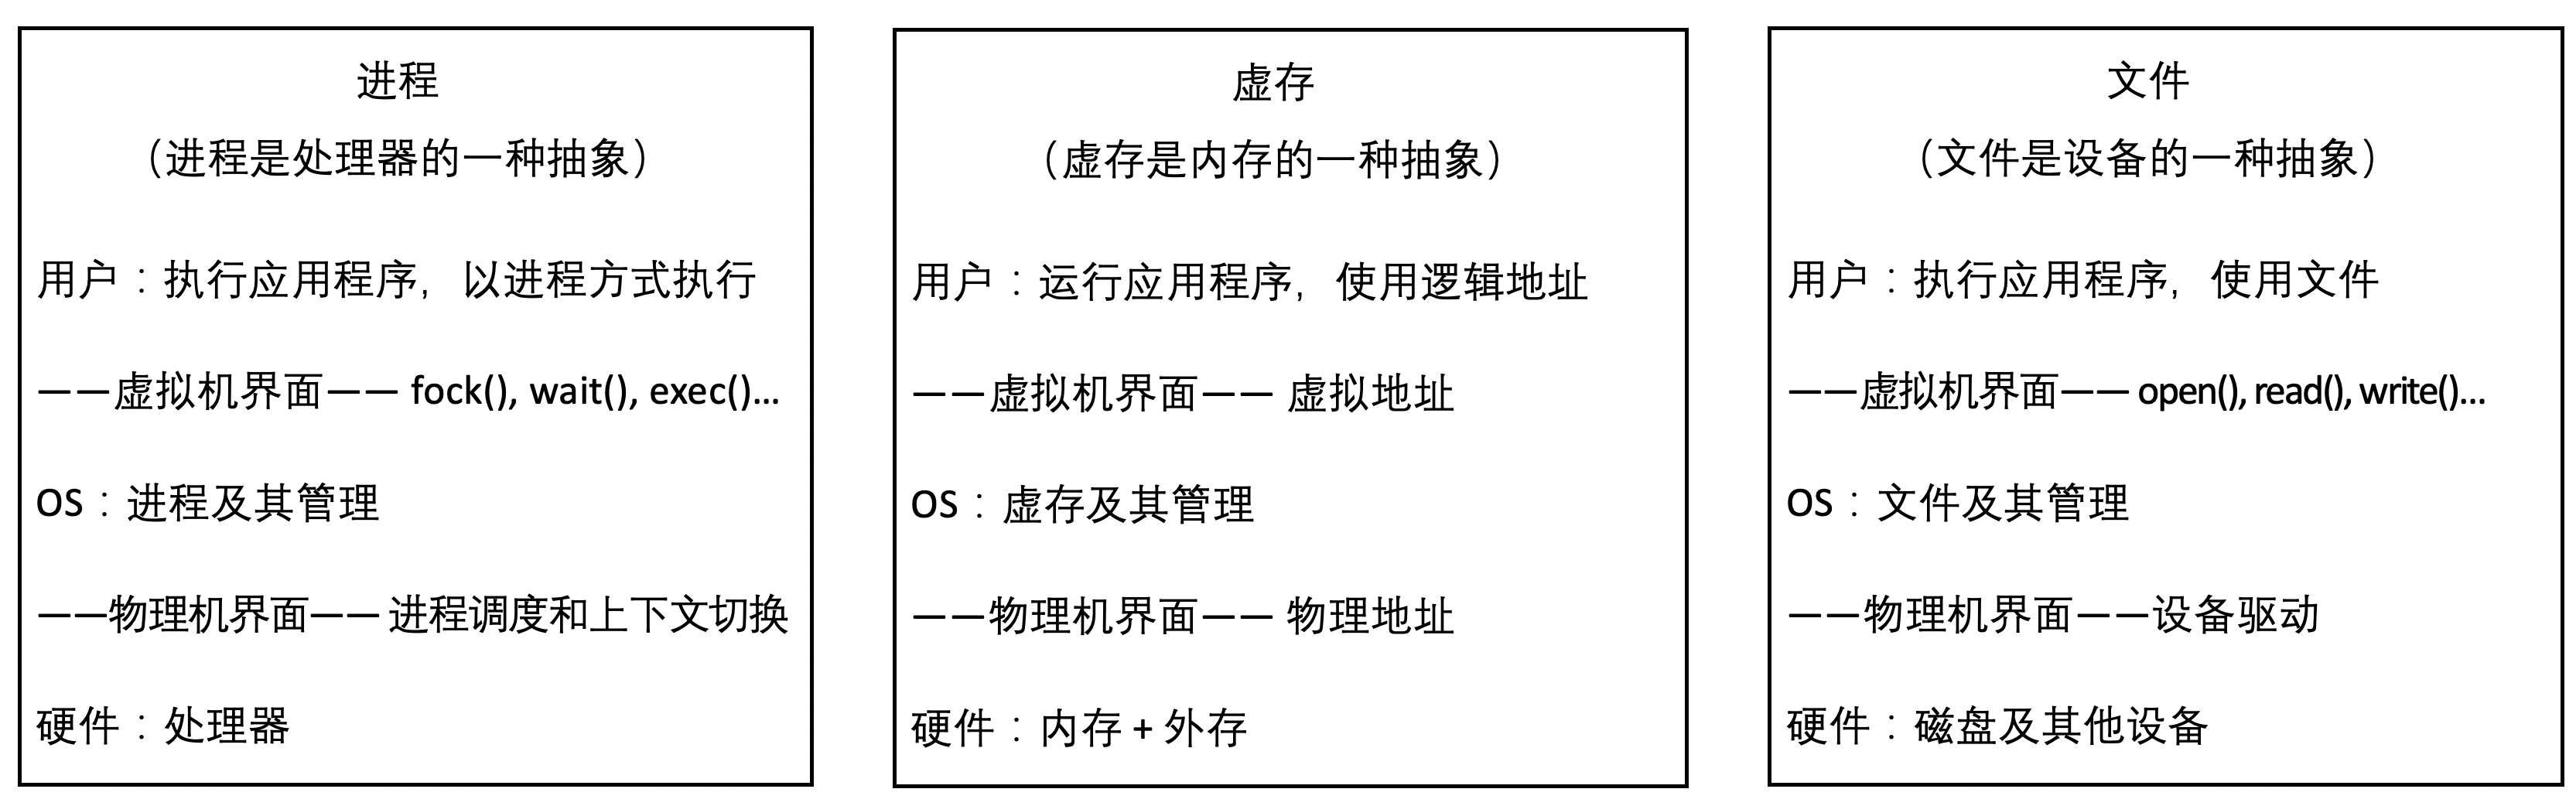
\includegraphics[width=0.95\textwidth]{img/1.3.1.2}
		\end{figure}
		\begin{itemize}
			\item 进程是对进入主存执行的程序在处理器上操作的状态集的一种抽象
			\begin{itemize}
				\item 它涉及执行程序及处理器,是\textbf{对处理器的一种抽象}
				\item 进程是并发和并行操作的基础
				\item 进程可以使用 \verb|fork()|、\verb|wait()|、\verb|exec()|等系统调用
				\item 进程的执行依赖于内存和设备上的信息资源
			\end{itemize}
			\item 虛存是\textbf{对主存的一种抽象}
			\begin{itemize}
				\item 本质上是在物理主存的基础上,通过结合 Cache、主存和外存的管理实现虚拟存储器,以提供一个比实际主存大得多的受保护的地址空间
				\item 在虚拟存储器上运行的进程不必考虑主存大小及地址映射的问题,且多个进程的虚存空间彼此隔离,具有很好的安全性
			\end{itemize}
			\item 文件是\textbf{设备的一种抽象}
			\begin{itemize}
				\item 通过将文件中的字节映射到存储设备的物理块中来实现文件抽象
				\item 应用程序可通过文件系统调用等来操纵和使用文件,而不必涉及设备的物理特性,不需要了解数据的存放位置和考虑信息如何传输
				\item 操作系统提供文件系统对文件进行统一管理,并调用设备驱动程序控制硬件设备按要求完成文件信息的 I/O
				\item 各类外部设备资源都可以抽象为文件,均可以按照文件系统调用访问,提供一致性的访问接口
			\end{itemize}
		\end{itemize}


		\subsection{程序控制的角度}
		\subsubsection{多道程序设计}
		多道程序设计允许多个程序同时进入计算机系统的主存,通过竞争处理器资源获得交替执行
		\begin{itemize}
			\item 宏观上看,这些程序是并发的
			\item 微观上看,这些程序是串行的,它们轮流占用 CPU 交替地执行
		\end{itemize}
		\begin{figure}[H]
			\centering
			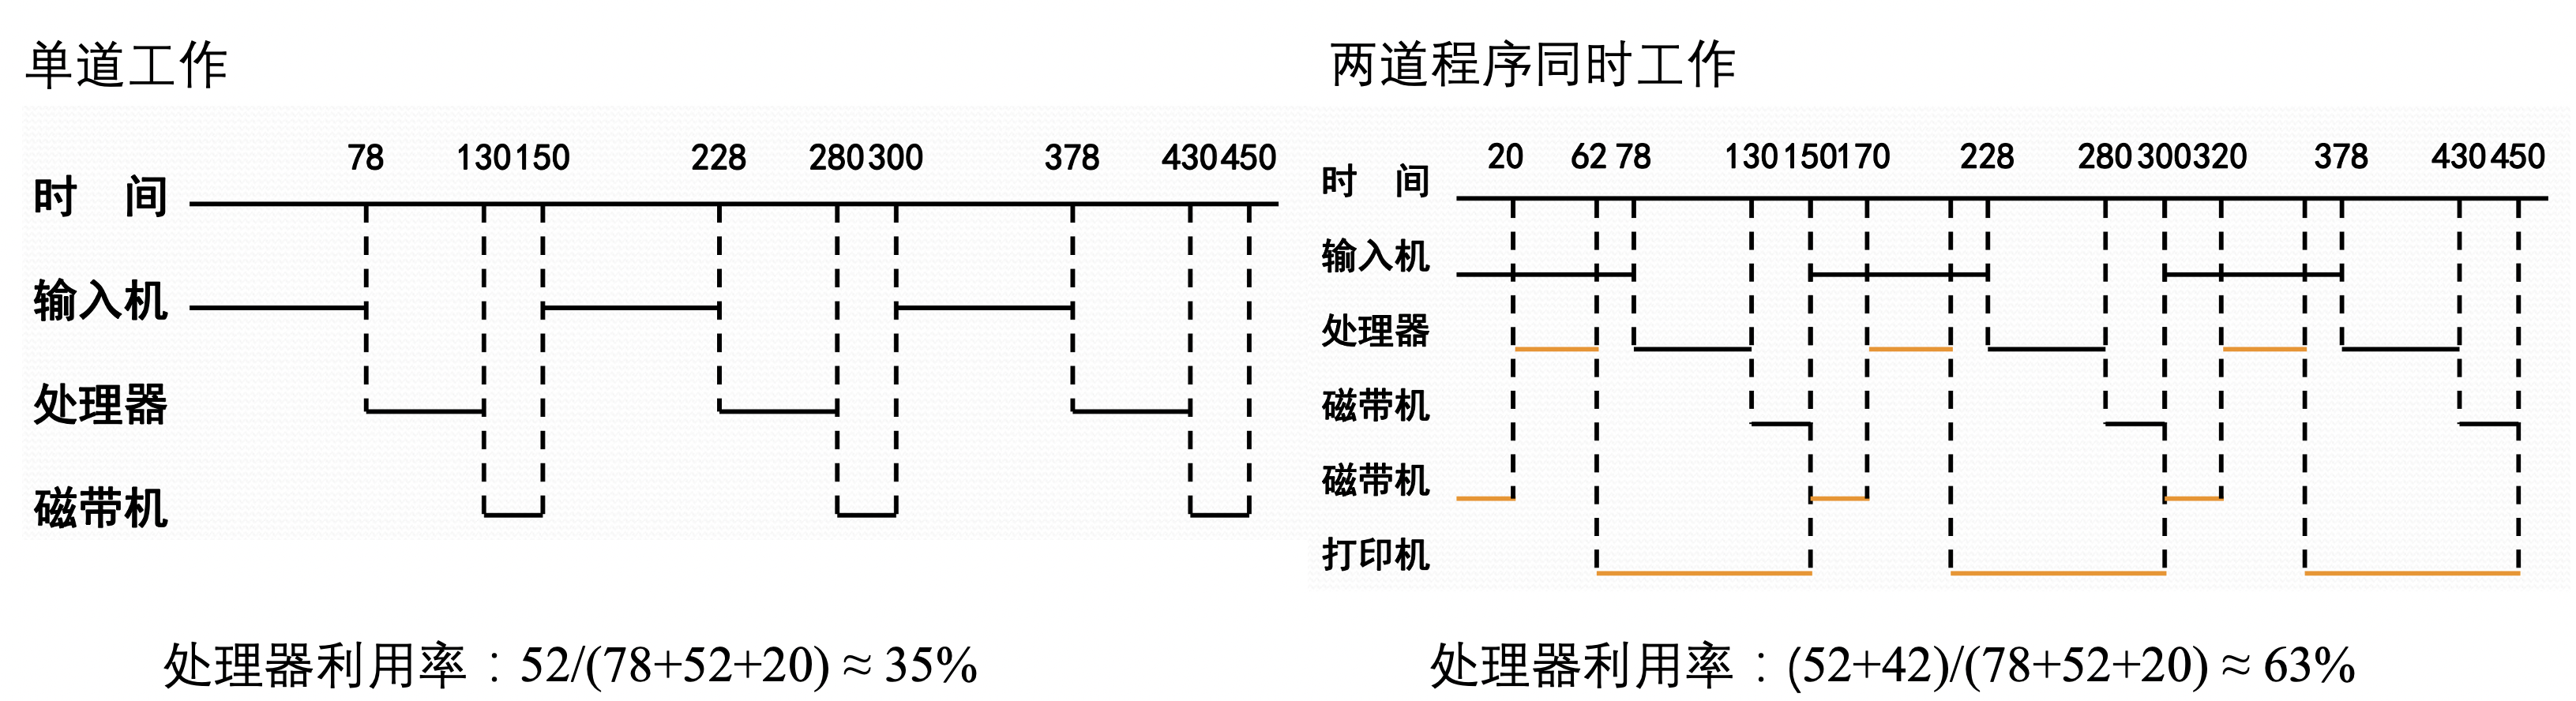
\includegraphics[width=0.95\textwidth]{img/1.3.2.1}
		\end{figure}

		多道程序设计的优点:
		\begin{itemize}
			\item 提高 CPU、主存和设备的利用率
			\item 提高系统的吞吐率,使单位时间内完成的作业数量增加
			\item 充分发挥系统的并行性,使设备与设备之间、CPU 与设备间均可并行工作
		\end{itemize}

		多道程序设计也不是道数越多系统效率越高,这依赖于 CPU 与设备的并行度
		\begin{itemize}
			\item 一旦多道程序在 CPU 或某个设备的使用上产生严重的堆积效应,就不会提高计算机系统的使用效率,反而会因为系统付出的管理开销导致性能下降
		\end{itemize}

		操作系统实现多道程序设计能够提高单位时间内处理的进程数,但不能提高单道作业的处理速度
		\begin{itemize}
			\item 反而会因为系统管理开销和排队使用资源导致单道作业处理时间的增加
			\item 即延长了单个作业的周转时间
		\end{itemize}

		\subsubsection{多道程序设计的实现要点}
		多道程序系统的实现:
		\begin{itemize}
			\item 为进入内存执行的程序建立管理实体:\textbf{进程}
			\item 操作系统应能管理与控制进程程序的执行
			\item 操作系统协调管理各类资源在进程间的使用
			\begin{itemize}
				\item 处理器的管理和调度
				\item 主存储器的管理和调度
				\item 其他资源的管理和调度
			\end{itemize}
		\end{itemize}

		多道程序设计的实现要点:
		\begin{itemize}
			\item 如何使用资源:调用操作系统提供的服务例程(如何陷入操作系统)
			\item 如何复用 CPU:调度程序(在 CPU 空闲时让其他程序运行)
			\item 如何使 CPU 与 I/O 设备充分并行:设备控制器与通道(专用的 I/O 处理器)
			\item 如何让正在运行的程序让出 CPU:中断(中断正在执行的程序,引入 OS 处理)
		\end{itemize}
		\begin{figure}[H]
			\centering
			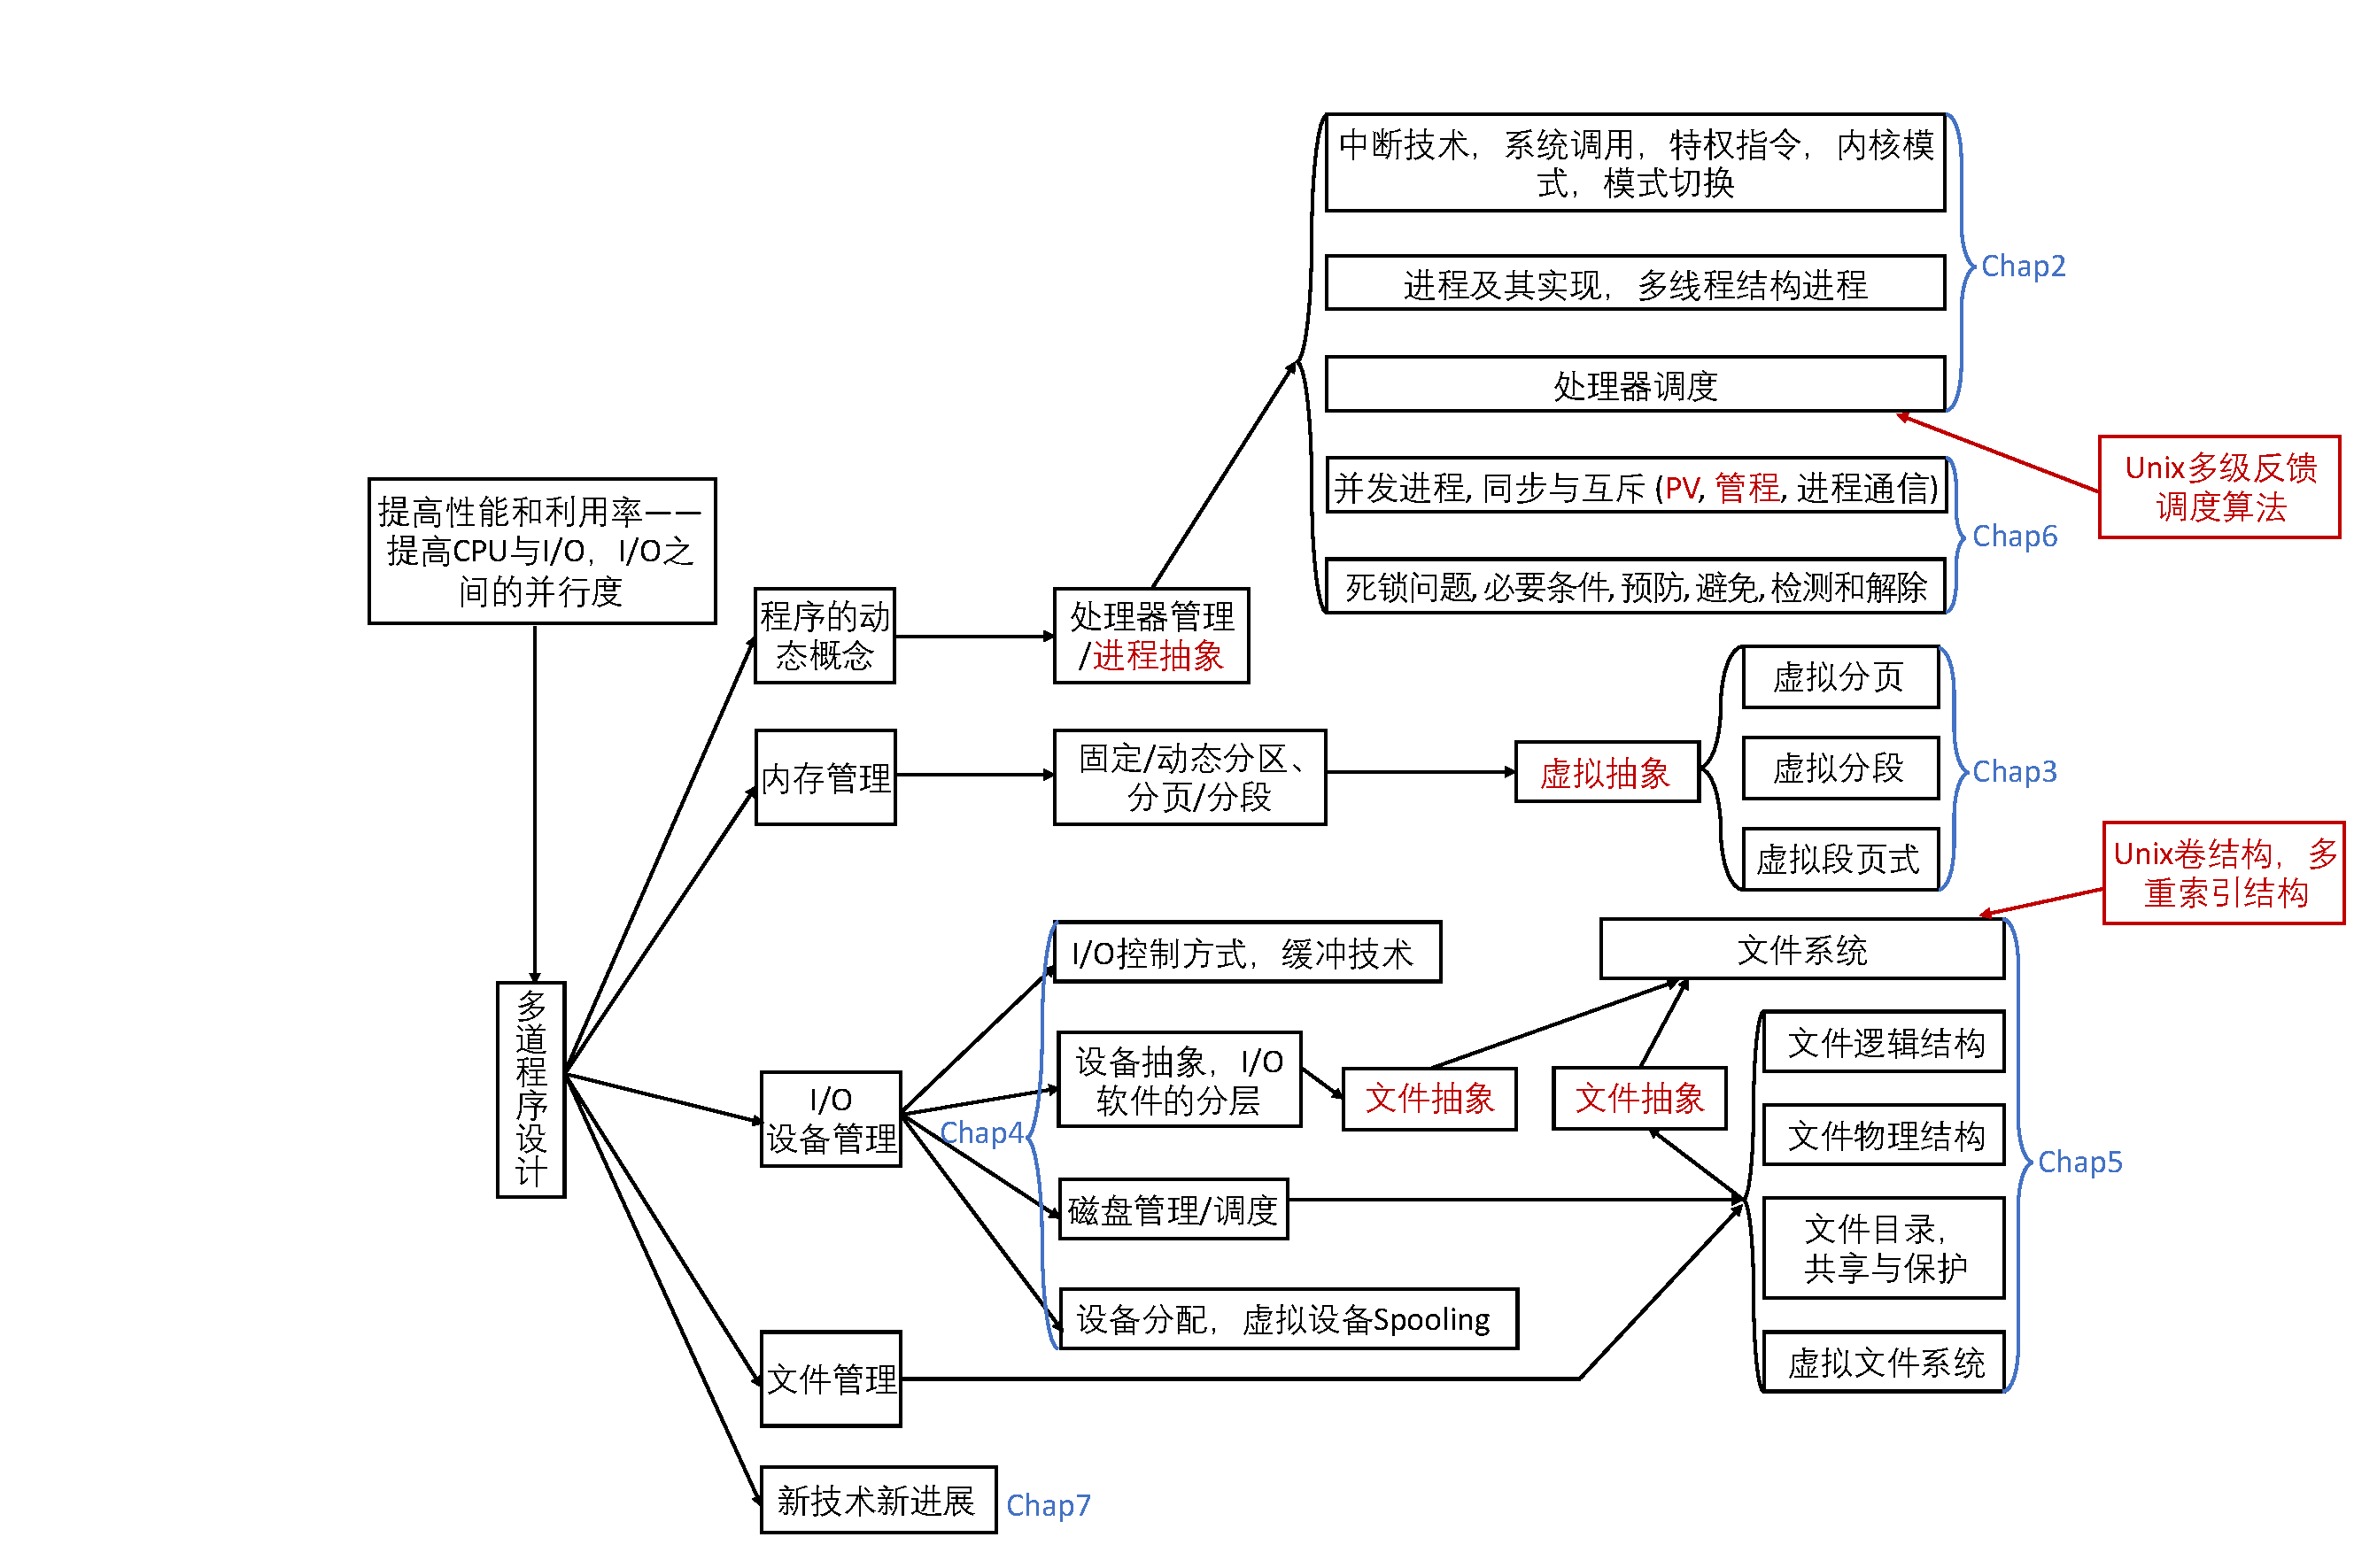
\includegraphics[width=0.95\textwidth]{img/1.3.2.2}
		\end{figure}


		\subsection{操作控制计算机的角度}
		\subsubsection{计算机操作控制方式}
		操作系统规定了合理操作计算机的工作流程,该工作流程是由操作系统接口——系统程序提供的,它为用户提供了操作控制计算机的所有服务

		操作系统提供脱机作业控制方式和联机作业控制方式两类作业级接口
		\begin{itemize}
			\item 脱机作业控制方式
			\begin{itemize}
				\item 执行过程:
				\begin{itemize}
					\item 操作系统提供作业说明语言
					\item 用户编写作业说明书,确定作业加工控制步骤,并与程序数据一并提交
					\item 操作员通过控制台输入作业
					\item 操作系统通过作业控制程序自动控制作业的执行
				\end{itemize}
				\item 例:批处理操作系统的作业控制方式,UNIX 的 shell 程序,DOS 的 bat文件
			\end{itemize}
			\item 联机作业控制方式
			\begin{itemize}
				\item 执行过程:
				\begin{itemize}
					\item 计算机提供终端(键盘/显示器)
					\item 用户登录系统
					\item 操作系统提供命令解释程序
					\item 用户联机输入命令,直接控制作业步的执行
				\end{itemize}
				\item 例:分时操作系统的交互控制方式
			\end{itemize}
		\end{itemize}


		\subsubsection{命令解释程序}
		无论是脱机作业控制方式还是联机作业控制方式,都需要提供对命令的解释处理

		命令解释程序是接受和执行一条用户命令并对作业加工处理的程序包

		当一个新的批作业被启动,或新的交互型用户登录进系统时,系统就自动地执行命令解释程序,负责读入控制卡或命令行,作出相应解释,并予以执行

		命令解释程序的处理过程
		\begin{itemize}
			\item 操作系统启动命令解释程序,输出命令提示符,等待键盘中断/鼠标点击/多通道识别
			\item 每当用户输入一条命令(暂存在命令缓冲区)并按回车换行时,申请中断
			\item CPU 响应后,将控制权交给命令解释程序,接着读入命令缓冲区内容,分析命令、接受参数,执行处理代码
			\item 前台命令执行结束后,再次输出命令提示符,等待下一条命令
			\item 后台命令处理启动后,即可接收下条命令
		\end{itemize}


		\subsection{人机交互的角度}
		\begin{itemize}
			\item 操作系统的人机交互(HCI)部分用于改善人机界面,为用户使用计算机提供良好的环境
			\item 人机交互设备包括传统的终端设备和新型的模式识别设备
			\item 操作系统的人机交互部分用于控制有关设备运行和理解执行设备传来的命令
			\item 人机交互功能是决定计算机系统友善性的重要因素,是当今操作系统研发热点
		\end{itemize}
		\subsubsection{人机交互的初期发展}
		交互式控制方式
		\begin{itemize}
			\item 行命令控制方式:1960 年代开始使用,一行一行进行编辑
			\item 全屏幕控制方式:1970 年代开始使用
		\end{itemize}
		斯坦福研究所提出的发展计划
		\begin{itemize}
			\item 始于 1960 年代,1980 年代广泛应用
			\item 强调人机交互的中心不是技术,也不是设备,而是人
			\item 代表性成果:鼠标、菜单与窗口控制(单窗口)
		\end{itemize}

		\subsubsection{WIMP界面}
		\begin{itemize}
			\item 缘起:70年代后期施乐公司(Xerox)的原型机 Star
			\item 特征:窗口(Windows)(多窗口)、图标(Icons)、菜单(Menu)和指示装置(Pointing Devices)为基础的图形用户界面 WIMP
			\item 得益:Apple 最初采用并大力推动
			\item 时间:1990 年代开始广泛使用
			\item 不足:不允许同时使用多个交互通道,从而产生人-机交互的不平衡
			\item Apple 的界面是 WIMP 的顶峰
		\end{itemize}


		\subsubsection{多媒体计算机}
		\begin{itemize}
			\item 缘起:1985 年的多媒体个人机
			\item 把音视频、图形图像和人机交互控制结合起来,进行综合处理的计算机系统
			\item 构成:多媒体硬件平台、多媒体操作系统、图形用户接口、多媒体数据开发工具
			\item 提供与时间有关的时变媒体(何时体现感觉更好)界面,既控制信息呈现,也控制何时呈现/如何呈现
			\item 人机交互界面需要使用多种媒体,同时支持多通道交互整合,改善用户体验
		\end{itemize}


		\subsubsection{虚拟现实系统}
		\begin{itemize}
			\item 缘起:1980 年代的虚拟现实新型用户界面
			\item VR 通过计算机模拟三维虚拟世界,根据观察点、观察点改变的导航和对周围对象的操作,来模拟临境的感觉
			\item 支持多通道交互整合,改善用户体验
			\item 支持用户主动参与的高度自然的三维 HCI,以及语音识别、头部跟踪、视觉跟踪、姿势识别等新型 HCI
			\item 容许用户产生含糊和不精确的输入
		\end{itemize}


		\subsection{程序接口的角度}
		\subsubsection{系统调用}
		系统调用是操作系统提供的程序接口,是现代操作系统内核提供的一系列具有预定功能的服务例程

		系统调用把应用程序的访问请求传送至内核,调用相应的服务例程完成所需处理,再将处理结果返回给应用程序

		\subsubsection{系统调用的实现}
		\begin{itemize}
			\item 操作系统实现系统调用功能的机制称为系统陷阱或系统异常处理机制
			\item 由于系统调用而引起处理器中断的机器指令称为陷入指令(trap),是非特权指令,在用户态下执行会产生 CPU 模式切换,即由用户态转换为内核态
			\item 执行陷入指令时,必须通过某种方式指明对应系统调用的功能号(每个系统调用事先规定的编号),大多数情况下还应附带有传递给相应服务例程的参数
			\item 系统调用的实现要点:
			\begin{itemize}
				\item 编写系统调用处理程序
				\item 设计一张系统调用入口地址表,每个入口地址指向一个系统调用的处理程序,并包含系统调用自带参数的个数
				\item 陷入处理机制需开辟现场保护区,以保存发生系统调用时的处理器现场
			\end{itemize}
			\begin{figure}[H]
				\centering
				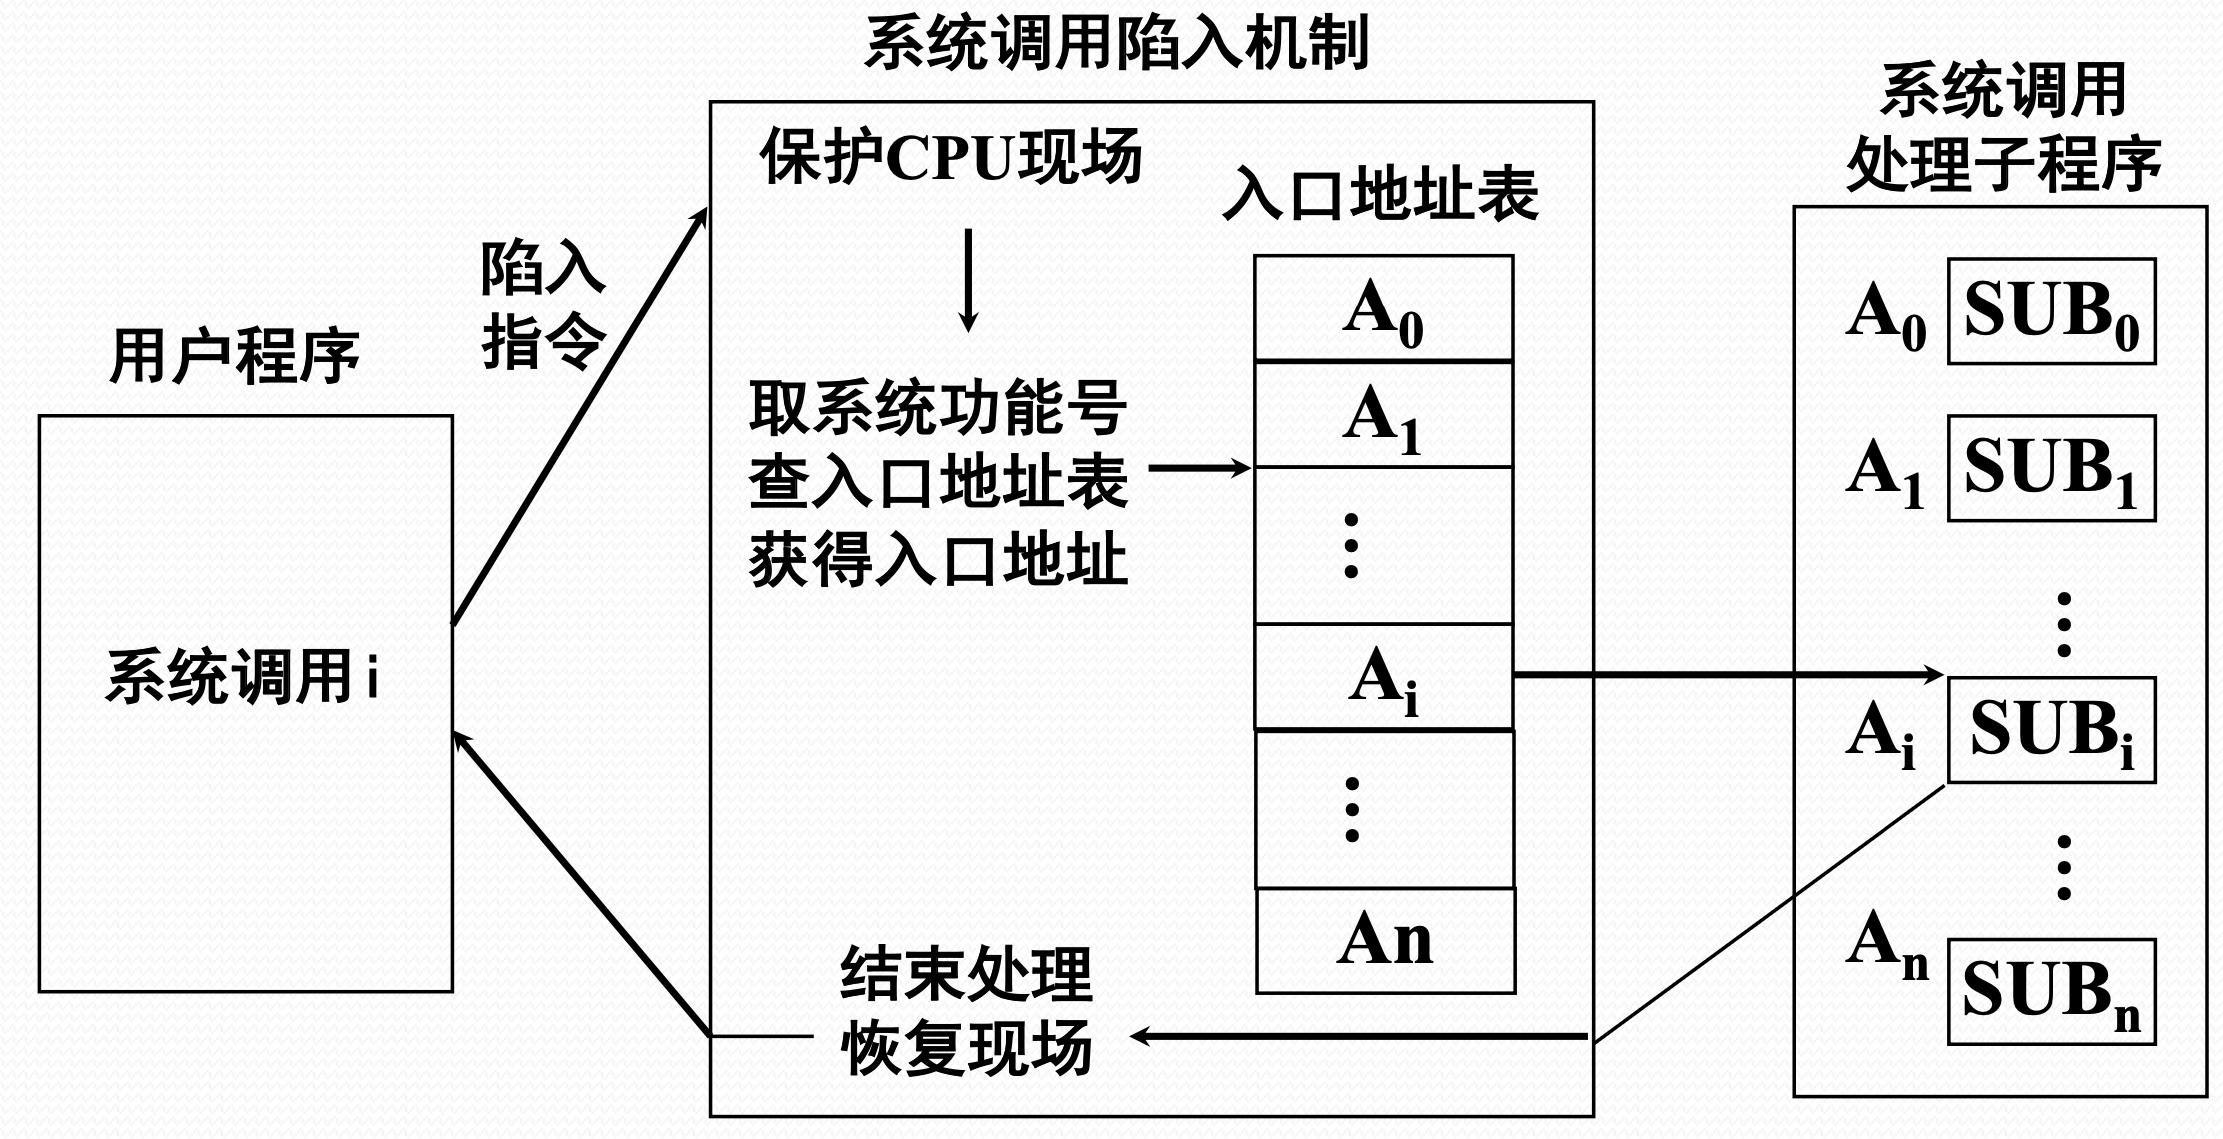
\includegraphics[width=0.65\textwidth]{img/1.3.5.2}
			\end{figure}
			\item 系统调用和函数调用之间的区别
			\begin{table}[H]
				\centering
				\begin{tabular}{|c|c|c|}
					\hline
					\textbf{} & 系统调用                 & 函数调用                                                             \\ \hline
					调用形式      & 按地址转向                & 功能号调用                                                            \\ \hline
					实现方式      & 用户态转换内核态,在内核态执行访问核心栈 & 用户态                                                              \\ \hline
					被调用代码位置   & 动态调用,服务例程位于操作系统内     & \begin{tabular}[c]{@{}c@{}}静态调用,调用程序和\\ 被调用程序在同一程序内\end{tabular} \\ \hline
					提供方式      & 由操作系统提供              & 编程语言提供                                                           \\ \hline
				\end{tabular}
				\end{table}
		\end{itemize}

		\subsection{系统结构的角度}
		\subsubsection{操作系统的工程化特征}
		\begin{itemize}
			\item 在计算机软件发展史上,操作系统是第一个大规模的软件系统
			\item 1960 年代,由操作系统开发所衍生的体系结构、模块化开发、测试与验证、演化与维护等研究,直接催生了软件工程这一新兴研究领域(另一个催生来源是数据库应用引发的需求与规格)
			\item 操作系统作为大型软件,结构设计是关键
		\end{itemize}

		\subsubsection{操作系统的结构设计}
		\begin{itemize}
			\item 操作系统构件:内核、进程、线程、管程等
			\item 设计概念:模块化、层次式、虚拟化
			\item 内核设计是操作系统设计中最为复杂的部分
			\begin{itemize}
				\item 内核是一组程序模块,作为可信软件来提供支持进程并发执行的基本功能和基本操作,通常驻留在内核空间,运行于核心态,具有直接访问硬件设备和所有内存空间的权限,是仅有的能够执行特权指令的程序
				\item 内核的功能
				\begin{itemize}
					\item 中断处理
					\item 时钟管理
					\item 短程调度
					\item 原语管理:原语是内核中实现特定功能的不可中断过程
					\begin{itemize}
						\item 原语由内核实现,系统调用由系统进程实现
						\item 例:通信原语、同步原语、I/O 设备原语
					\end{itemize}
				\end{itemize}
				\item 内核的属性
				\begin{itemize}
					\item 内核是由中断驱动的
					\item 内核是不可抢占的
					\item 内核可以在屏蔽中断状态下进行
					\item 内核可以使用特权指令
				\end{itemize}
				\item 操作系统的内核设计目前有以下四种方式:
				\begin{itemize}
					\item 单内核:内核中各部件杂然混居的形态,始于 1960 年代,广泛使用,例如 Unix/Linux 和 Windows(自称采用混合内核的 CS 结构),单内核导致内核会非常大
					\item 微内核:仅将所有应用必须的核心功能放入内核,其他功能都在内核之外,由在用户态运行的服务进程实现,强调结构性部件与功能性部件的分离,大部分操作系统研究都集中在此,效率不高
					\item 混合内核:微内核和单内核的折中,较多组件在核心态中运行,以获得更快的执行速度
					\item 外内核:尽可能减少内核的软件抽象化和传统微内核的消息传递机制,使得开发者专注于硬件的抽象化;部分嵌入式系统使用
				\end{itemize}
			\end{itemize}
		\end{itemize}

		\paragraph{操作系统实现的一种结构层次}~{}

		\begin{figure}[H]
			\centering
			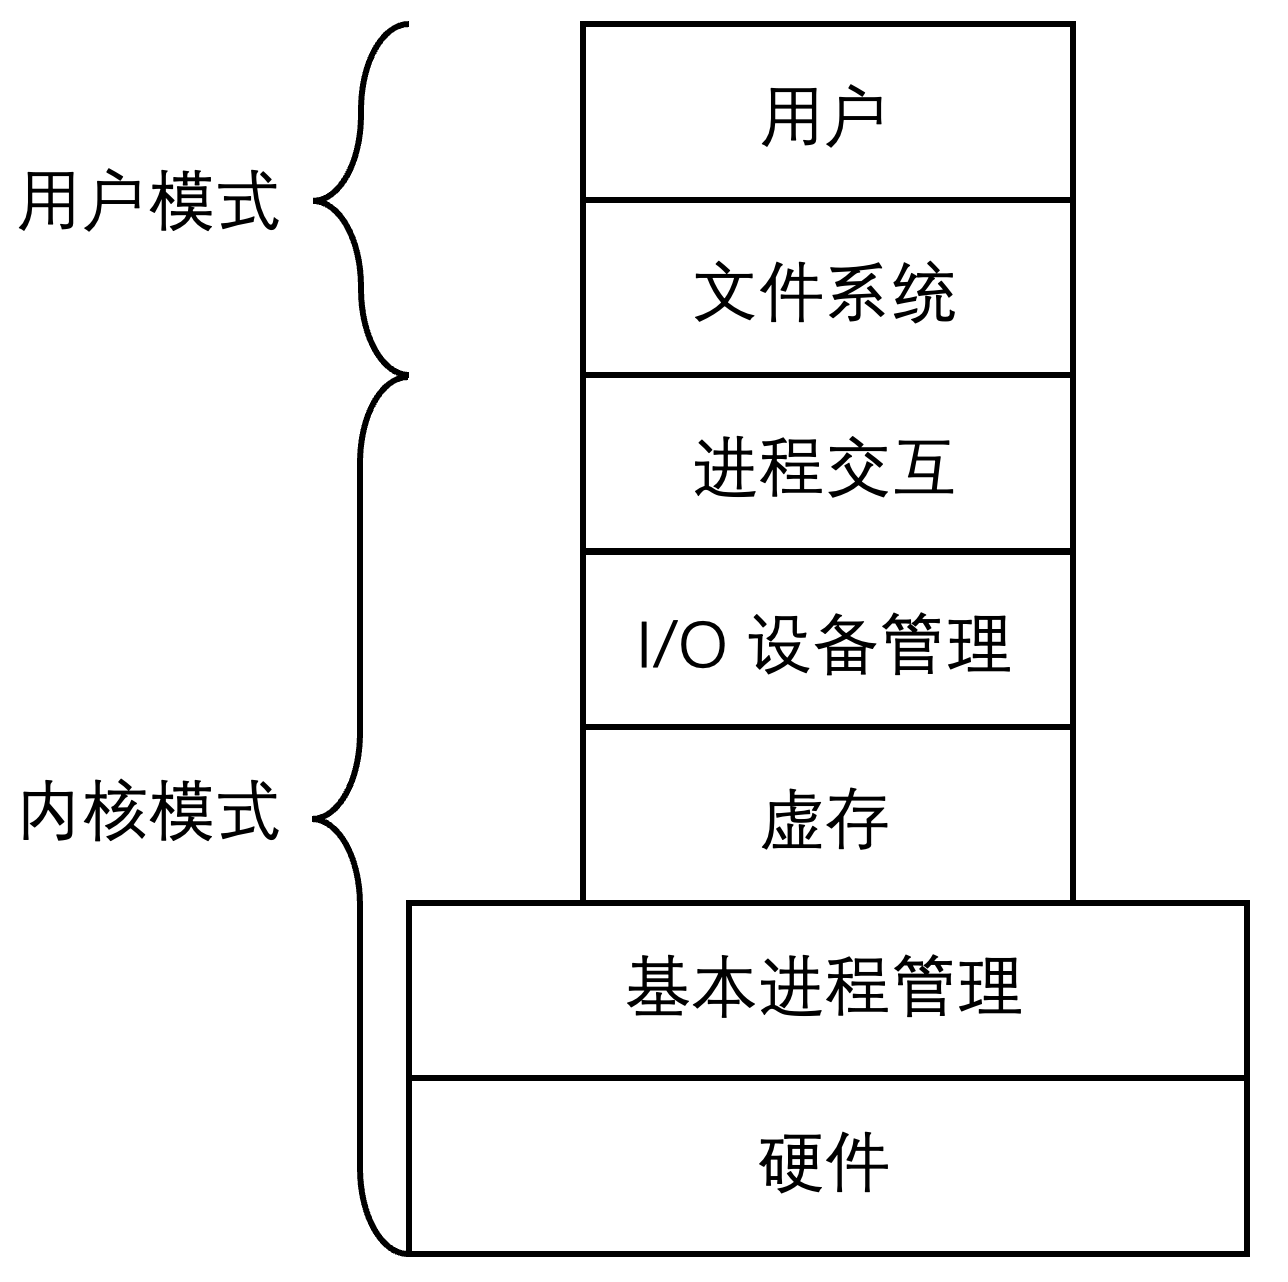
\includegraphics[width=0.65\textwidth]{img/1.3.6.1}
		\end{figure}
		现在文件系统也会划归到内核中

		\paragraph{操作系统实现的第二种结构层次}~{}

		过程机制、指令解译、电路执行是由硬件完成,实现中断等机制

		当前操作系统除了硬件电路以外都是由操作系统管理
		
		\begin{figure}[H]
			\centering
			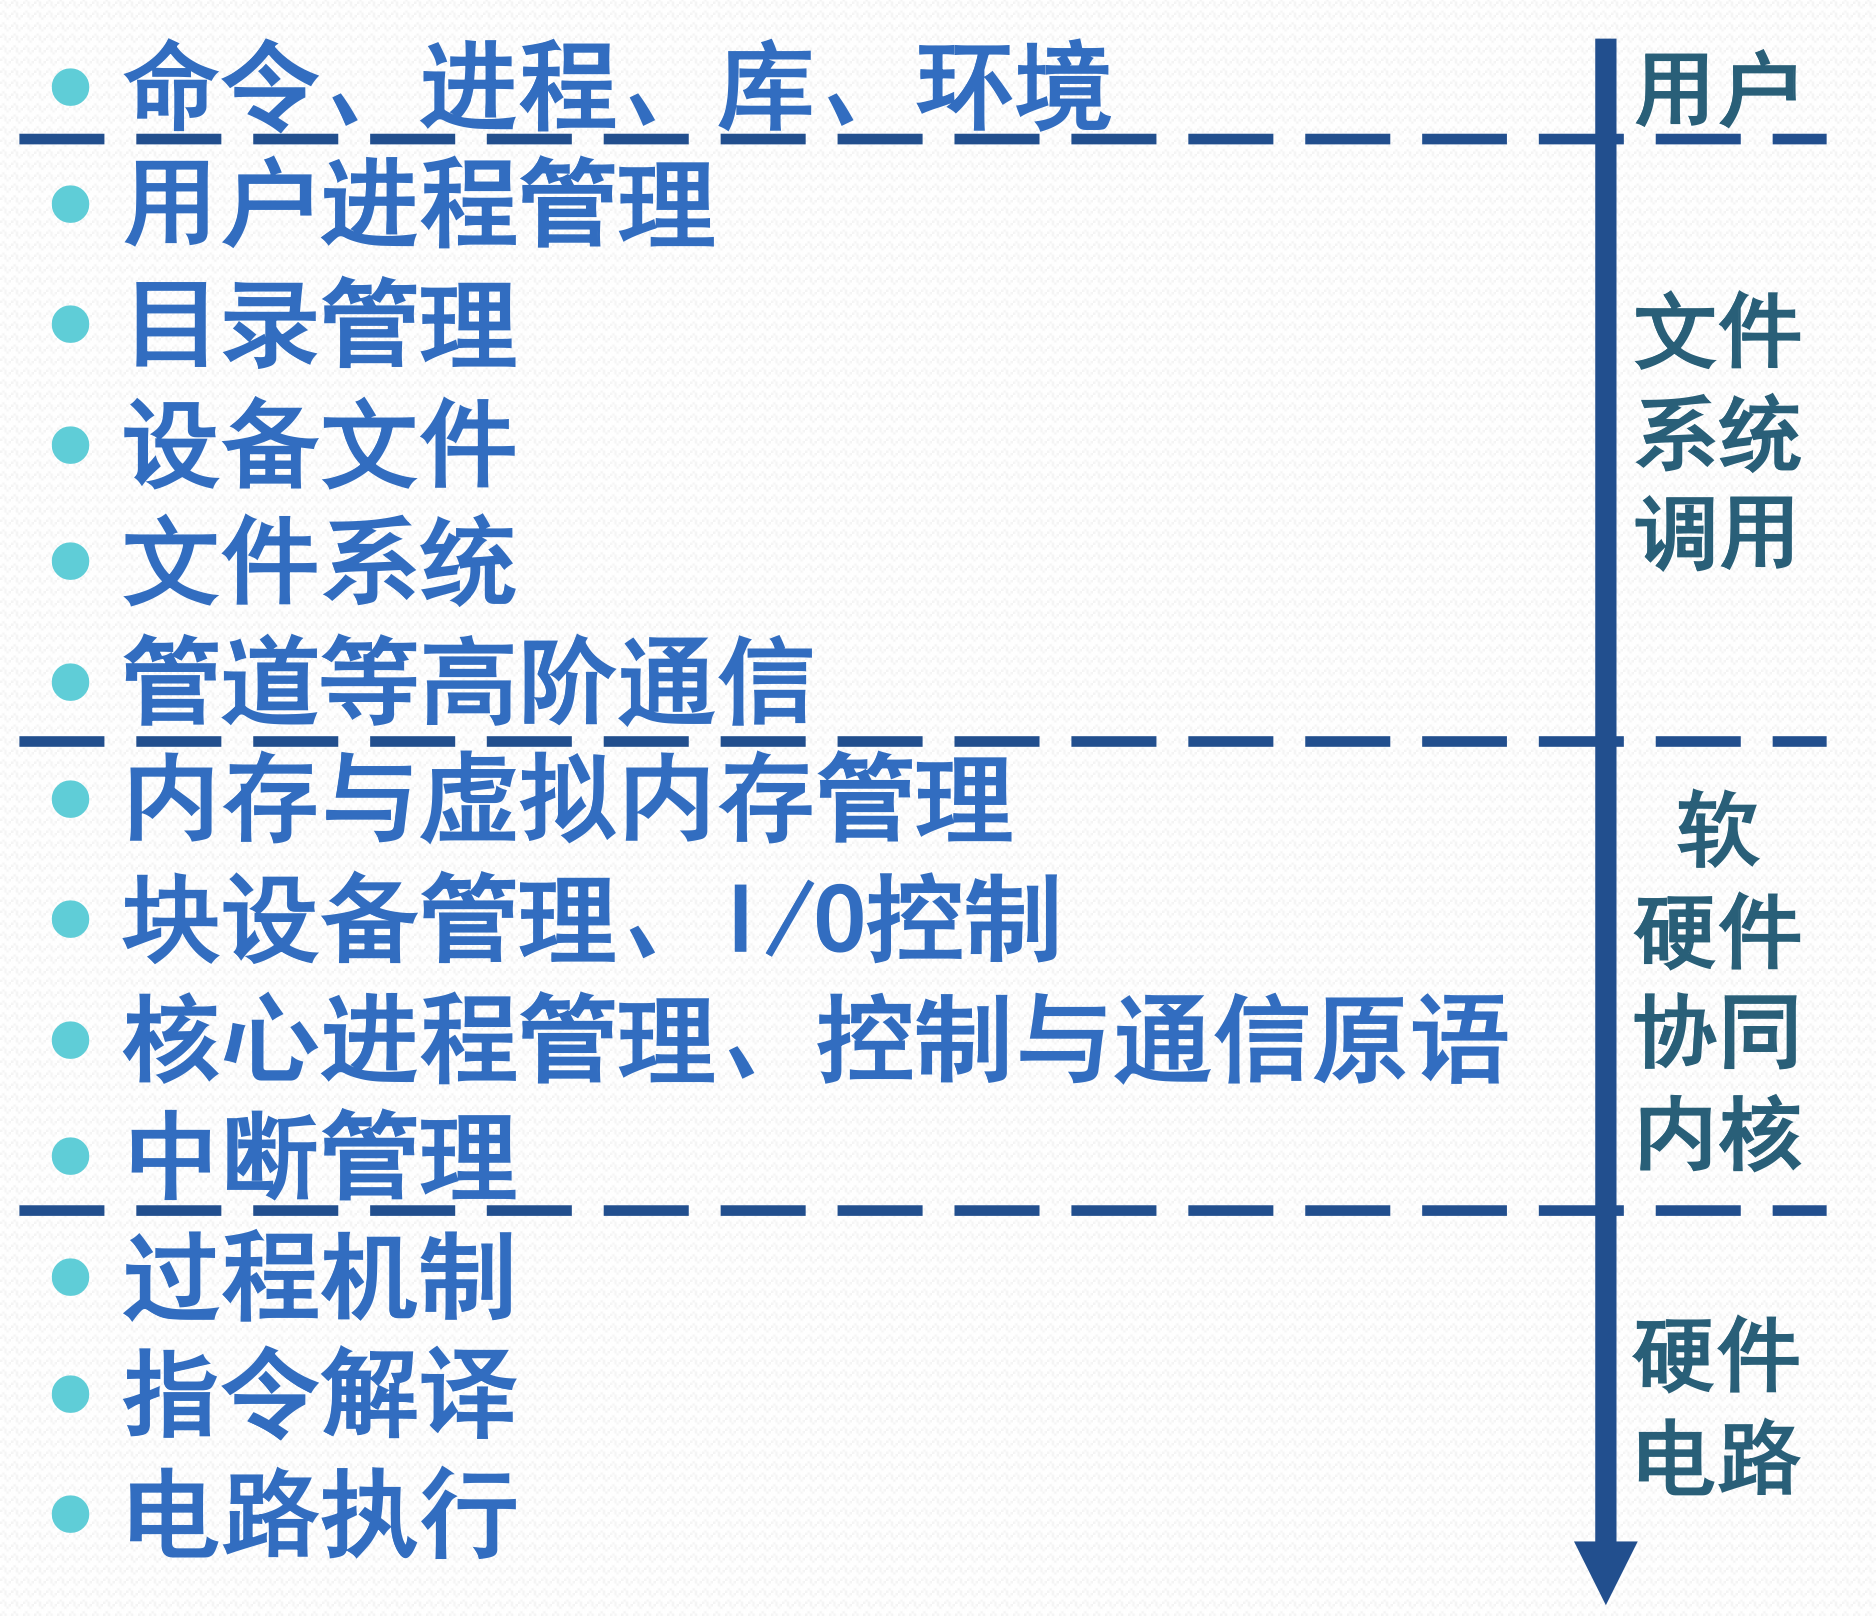
\includegraphics[width=0.65\textwidth]{img/1.3.6.2}
		\end{figure}

\end{document}



